\chapter{Search for SUSY in a final state with at least two hadronically decaying tau leptons}
\label{ch:analysis}
\epigraph{\emph{"Let us choose for ourselves our path in life, and let us try to strew that path with flowers."}}{Emilie du Chatelet}
%“All sorts of things can happen when you’re open to new ideas and playing around with things.” — Stephanie Kwolek


%\textcolor{purple}{have to still include CMS result in the review of the analysis? might be able to compare that to the SUSY2022 slides on CMS search!\\}

This chapter is describing a search for supersymmetric particles in a final state with at least two hadronically decaying tau leptons.  This search has been the author's main project and has been the author's sole responsibility.  This work has been published as \ac{ATLAS} conference note \cite{AnalysisConf} and was presented at ICHEP2022 through a poster contribution by the author \cite{ICHEP2022Poster}.
%Have to cite this: https://agenda.infn.it/event/28874/contributions/175844/
An introduction to the theoretical model of interest to this search, together with a short motivation of the model is given in section \ref{sec:analysis:intro}.  In section \ref{sec:analysis:previous}, an overview of other experimental searches for this model is given.  The strategy of the analysis discussed here is given in section \ref{sec:analysis:strategy},  with an overview of the considered samples (\ref{sec:analysis:samples}) and the selection process employed in this search (\ref{sec:analysis:eventselection}).  Definitions of the analysis objects are given in section \ref{sec:analysis:objectDef}, followed by the signal region optimisation (\ref{sec:analysis:sroptimisationSection}) and  background estimation (\ref{sec:analysis:bkgestimation}).  An overview of the considered uncertainties is given in section \ref{sec:analysis:systematics}.  Before discussing the final results and interpretation in section \ref{sec:analysis:results} and \ref{sec:analysis:interpretation},  the statistical concepts relevant for this analysis (\ref{sec:analysis:stats}) are summarised.   
The described search has then been combined with a search for the same model in a different final state.  This search has not been performed by the author but the statistical combination has been; therefore a brief overview of this orthogonal search is given in section \ref{sec:analysis:os}, before illustrating the gain of the statistical combination of the analyses in section \ref{sec:analysis:combination}.

\section{Introduction and theoretical motivation}
\label{sec:analysis:intro}
Supersymmetry is a promising extension of the \ac{SM},  with a multitude of possible production mechanism of supersymmetric particles at the \ac{LHC}.  In hadron-hadron collisions,  the production of particles through strong interactions is the dominant mechanism.  As can be seen in Figure \ref{fig:analysis:xsec}, the strong production of supersymmetric particles has a larger cross section than an electroweak production through gauginos or sleptons.  However, if strongly produced particles (gluinos and squarks) are heavy,  electroweak production cross sections can become the leading production mode of \ac{SUSY} particles at the \ac{LHC}.  Given the latest status of strong and third generation squark searches as discussed in section \ref{sec:theory:biggerPicture},  gluinos and squark masses are expected to be larger than 1 TeV in most cases. This is motivating the investigation of electroweak production modes of \ac{SUSY} as presented within this thesis. 


\begin{figure}
\centering
\includegraphics[width=0.7\linewidth]{figures/SUSY_xsecs_13TeV_overview.pdf}
\caption{Cross section comparison in 13 TeV proton-proton collisons \cite{SUSYXSecWorkingGroup,XSecCalcPaper} \label{fig:analysis:xsec}}
\end{figure}
%
This electroweak production of \ac{SUSY} particles includes the production of charginos and neutralinos.  Assuming R-Parity conservation (see equation \eqref{eq:theory:rparity}),  \ac{SUSY} particles are pair-produced and the lightest \ac{SUSY} particle is stable.  A stable lightest supersymmetric particle can be a candidate for Dark Matter. 
In the search for \ac{SUSY} particles described here,  a simplified model (Figure \ref{fig:analysis:simplifiedmodel}) is considered in order to optimise search regions and interpret the results. 
The lightest Chargino (\Cone) is produced together with the next-to-lightest neutralino (\Ntwo).  This can happen through a multitude of proton-proton interactions,  which is visualised through the larger gray shaded area. 

\begin{figure}[!htpb]
\centering
\includegraphics[width=0.45\linewidth]{figures/C1N2-tautautauvN1N1-stausnu.pdf}
\caption{Feynman diagram of the simplified supersymmetric model considered in this thesis \label{fig:analysis:simplifiedmodel} \cite{AnalysisConf}}
\end{figure}
In this simplified SUSY model,  the \Ntwo and \Cone are assumed to be mass degenerate and Wino dominated.  The \Cone, \Ntwo consecutively decay via a \stau or \sneutrino into the lightest,  bino-like neutralino (\None).  In many parameter configurations of \ac{SUSY},  third generation sleptons can be the lightest sleptons \cite{SUSYPrimer},  motivating the \Cone \Ntwo decay via \stau or \sneutrino. The \None is assumed to be the lightest supersymmetric particle and therefore stable under R-parity conservation and a \ac{DM} candidate.  
The \Stau and \sneutrino masses are fixed through a parameter $x$ as described in equation \eqref{eqn:analysis:staumass}  (adapted from \cite{DiTauC1N2_2018}).  In the investigation of the model considered here,  this parameter is fixed to 0.5.  As discussed in section \ref{sec:theory:susy},  the gauge and mass eigenstates of the \stau 's can differ. In this simplified model,  $\tilde{\tau}_L$ and $\tilde{\tau}_R$ are assumed to be mass-degenerate.  
\begin{equation}
m_{\tilde{\tau}/ \tilde{\nu_\tau}} = m_{\tilde{\chi}_1^0} + x * \Delta m(\tilde{\chi}_2^0 - \tilde{\chi}_1^0)
\label{eqn:analysis:staumass} 
\end{equation}
%
In this simplified model,  the \Cone decays via a \Stau and \nutau or \sneutrino and $\tau$ further into either a $\tau$ or \nutau and a \None. In both cases,  one neutrino,  one tau and one \ac{LSP} are the final state of this leg of the simplified model.  The \Ntwo decays via a \stau or \sneutrino into a pair of two $\tau$ leptons or $\tau$ neutrinos.  In order to achieve a final state with at least two hadronically decaying tau leptons,  the \Ntwo has to decay via a \stau. 

%Light electroweakinos up to around 1 TeV are of phenomenological interest -- \textcolor{red}{references in the all hadronic paper are looking at wino LSP - not the case here!}
%%
Supersymmetric models with light sleptons,  such as the \stau considered in the discussed model,  can offer a Dark Matter candidate that can be compatible with the observed relic Dark Matter density,  thanks to possible co-annihilation of neutralinos via these light sleptons \cite{Coannihilation}. 
Since lepton flavour universality is not a fixed symmetry in the \ac{SM} and \ac{SUSY},  considering all lepton flavours in searches for new physics is crucial.
%\textcolor{purple}{want to further discuss any other motivations of this model? - are there any gambit or other references?}
%%https://link.springer.com/article/10.1007/JHEP04(2020)165
%%https://journals.aps.org/prl/abstract/10.1103/PhysRevLett.86.3484
%%https://journals.aps.org/prd/abstract/10.1103/PhysRevD.56.4424
%
%%\textcolor{gray}{\begin{itemize}
%%	\setlength\itemsep{-0.5em}
%%\item introduction of simplified model 
%%\item derivation/assumptions on that from pMSSM
%%\item Dark Matter reasoning
%%\item stau coannihilation
%%\item GAMBIT motivations 
%%\end{itemize}
%%}



\section{Previous model investigations}
\label{sec:analysis:previous}
The above described simplified model has been previously investigated with the \ac{ATLAS} detector during Run-1 \cite{Run1analysis,Run1combination} and most recently using partial Run-2 data \cite{DiTauC1N2_2018}. 
Within the partial Run-2 data analysis, a search for the \Cone \Ntwo production described above,  as well as a simplified model of \Cone pair production decaying via staus,  was considered. 
In the analysis,  a final state with at least two hadronically decaying taus of opposite electric charge was considered. 
No significant excesses were observed,  leading to an interpretation in the \Ntwo, \None mass plane given in Figure \ref{fig:previous:mnonentwo}.  For a massless \ac{LSP},  \Ntwo masses up to 760 GeV were excluded. 
In addition to mass points with a fixed stau and sneutrino mass parameter $x$ (as defined in equation \eqref{eqn:analysis:staumass}),  two benchmark points were investigated with $x$ varying between and 0.05 and 0.95.  The $CL_s$ significance for a scenario with lower mass splitting,  investigating a signal point with \None mass of 100~GeV and \Ntwo mass of 250 GeV is shown in Figure \ref{fig:previous:xvariation}.  The $CL_s$ significance is here used to express the confidence level connected with the $CL_s$ value - a detailed discussion of the statistical concepts behind the model-dependent exclusion discussed here is given in section~ \ref{sec:analysis:stats}.

\begin{figure}[htpb!]
\centering
\subfloat[\label{fig:previous:mnonentwo}]{\includegraphics[width=0.49\linewidth]{figures/C1N2SS/previousAnalyses/fig_07b.pdf}}
\subfloat[\label{fig:previous:xvariation}]{\includegraphics[width=0.49\linewidth]{figures/C1N2SS/previousAnalyses/fig_08c.pdf}}
\caption{Results of previous model investigations in partial Run-2 data \cite{DiTauC1N2_2018} \label{fig:analysis:previousresults}. In its \Mnone vs \Mntwo interpretation,  as well as for a benchmark point in dependency of the stau mass splitting parameter $x$. }
\end{figure}

As can be seen in both exclusion plots,  the mass point (\Ntwo,\None) = (250,100) GeV is excluded by the analysis.  For no values of $x$ the $CL_s$ significance has dropped below the dashed line,  highlighting a confidence level below 95\%.  
Even though there is a visible dependency on the stau mass parameter $x$ on the sensitivity of the analysis,  this dependency does not change the conclusion of the model investigation. This is a further motivation to continue with an assumption of $x = 0.5$ within the analysis described in the following.  \\
The \acs{CMS} Collaboration has performed a search for the production of a \Cone and \Ntwo with a consecutive decay via sleptons \cite{CMSDitauGaugino} that includes a decay via stau leptons as described above. This search in 2016-2018 proton-proton collisions used multiple final states,  including multi-leptonic final states with a light lepton and at least one hadronically decaying tau.  A parametric neural network was used to enhance the sensitivity to the supersymmetric particle signal. No significant excesses have been observed in this search,  leading to the exclusion of \Ntwo masses up to 970 GeV for massless \None. 
The larger available statistics offered by the full LHC Run-2 dataset used within this thesis allows for an investigation of the previously unaccessible regions of phase space,  particularly towards higher \Cone masses and low mass splittings between \Cone and \Ntwo. The same-sign di-tau final state considered in this thesis will offer a orthogonal approach to the analyses considered before, with different background compositions than in a opposite sign di-tau final state.  The orthogonality of both approaches will significantly increase the phase space coverage of the model. %%%The enhanced statistics compared to the previous \ac{ATLAS} investigation of the simplified model will significantly extend the 
%%%%%%%%%%%%TODO%%%%%%%%%%%%%%%%%%%%%%%%
%\textcolor{purple}{highlight why its beneficial to include the SS final state, want to talk about the CMS result, too?}
%\textcolor{blue}{might want to compare that to a via slepton production as well?}
%\textcolor{purple}{look at the latest CMS result here: 2106.14246}
% https://arxiv.org/pdf/2106.14246.pdf

%\textcolor{gray}{\begin{itemize}
%	\setlength\itemsep{-0.5em}
%\item partial run-2 ATLAS result -- done
%\item CMS result
%\item limitations of previous results -- not discussed
%\item motivation of the SS extension next to OS final state -- not discussed
%\item show exclusion limit in dependence of x to motivate choice of x -- done?
%\end{itemize}
%}
\section{Analysis strategy}
\label{sec:analysis:strategy}
The simplified supersymmetric model presented in section \ref{sec:analysis:intro} has been investigated in a final state with at least two hadronically decaying tau leptons,  with the leading two taus of same electric charge.  
Apart from the hadronic tau final state,  the composition of \ac{SM} backgrounds largely depends on the additional objects in the event.  One significant difference in the composition of the collision events considered is the amount of missing transverse momentum present.
In regions with low and moderate amount of \Met, the dominant processes have \Met originating from single neutrinos or from mis-measurements.  \ac{SM} decays involving more neutrinos in the decay chain can lead to higher \Met. 
Differences in the magnitude of missing momentum in the event are directly connected with differences in the assumed masses of the supersymmetric particles.  The lightest neutralino, \None ,  will not decay into \ac{SM} particles,  nor interact with the detector material.  Therefore the magnitude of missing transverse energy reconstructed is connected with the mass and momentum of the \None.
To target different mass ranges of the simplified model,  two strategies have been designed.  One targeting low \None masses as well as low mass splittings between the \None and \Cone,  a second scenario targets high \None and \Cone masses,  leading to higher \Met. 

\begin{figure}[!htpb]
\centering
\subfloat[Multi-jet \label{fig:feynmans:multijet}]{\includegraphics[height=3cm]{figures/FeynmanDiagrams/multijet.pdf}}
\subfloat[Multiboson]{\includegraphics[height=3cm]{figures/FeynmanDiagrams/WZdilep.pdf}}
\subfloat[Top \label{fig:feynmans:ttbar}]{\includegraphics[height=3cm]{figures/FeynmanDiagrams/ttbar.pdf}}\\
\subfloat[W+jets \label{fig:feynmans:wjets}]{\includegraphics[height=3cm]{figures/FeynmanDiagrams/wjetslep.pdf}}
\subfloat[Z+jets \label{fig:feynmans:zjets}]{\includegraphics[height=3cm]{figures/FeynmanDiagrams/zjetstau.pdf}}
\subfloat[Higgs \label{fig:feynmans:higgs}]{\includegraphics[height=3cm]{figures/FeynmanDiagrams/ttH.pdf}}\\
\caption{Overview of \ac{SM} processes contributing to a di-tau final state \label{fig:bkgestimation:feynmanOverview}}
\end{figure}

An overview of the \ac{SM} processes considered,  which can enter a di-tau final state is given in Figure \ref{fig:bkgestimation:feynmanOverview}. Here only a few selected feynman diagrams for these \ac{SM} processes are shown for illustration.
\textit{Multi-jet} processes include all QCD processes that end up in a final state with multiple jets.  The example shown in Figure \ref{fig:feynmans:multijet} shows a gluon fusion process.  The parton showering of these gluons into jets can lead to jets that are mis-identified as hadronically decaying tau leptons.  In \textit{Multi-boson} processes,  the associate production of multiple \ac{SM} $Z$ or $W$ bosons can lead to a final state with two tau leptons.  This is governed by the branching ratios of the $Z$ and $W$ boson decaying into tau leptons ($3.37\%$  and $11.38\%$ respectively \cite{PDG2022}).  This also applies to the associate production of $W$ or $Z$ bosons with jets,  as shown in Figures \ref{fig:feynmans:wjets} and \ref{fig:feynmans:zjets}.  In this single boson productions, at least one of the hadronic taus in the final state is a so-called \textit{fake tau},  originating from mis-identified jets. 
Processes associated with top quarks like the top quark pair production shown in Figure \ref{fig:feynmans:ttbar} can contribute to a di-tau final state both through hadronically decaying taus or mis-identified, fake taus.  This is due to the decay of the top quarks into a bottom quark and $W$ boson,  which can consecutively decay into a tau lepton.
In this thesis,  all \ac{SM} processes containing a Higgs boson,  even in association with top quarks as depicted in Figure \ref{fig:feynmans:higgs} are considered as \textit{Higgs} processes.  Similar to the top associated processes,  whether the final state tau objects are misidentified jets or tau leptons depends on the decay of the Higgs boson as well as the top quark decay.  The background estimation techniques described within section \ref{sec:analysis:bkgestimation} do not separate the backgrounds based on the number of fake taus, but rather based on the \ac{SM} processes as highlighted in Figure \ref{fig:bkgestimation:feynmanOverview}.


\section{Data and simulation samples}
\label{sec:analysis:samples}
An introduction to Monte Carlo simulation principles used in particle physics as well as an overview of the Monte Carlo generators of importance to this thesis was given in section \ref{sec:DAQ:MC}.  In the following,  details about the simulated events used in this analysis for the various \ac{SM} backgrounds as well as \ac{SUSY} signal is given.

For all samples considered here,  \texttt{PYTHIA8} was used to overlay simulated soft QCD processes.  This simulation is usually performed before the exact pile-up conditions in data are known.  Therefore the simulation is corrected through re-weighting of events to match the year-by-year pileup conditions described in section \ref{sec:ExpSetup:LHC}. 

\textbf{Top} related processes include top quark pair production (\ttbar) as well as single-top production via s-, t- and Wt-channels. These processes were simulated using  \texttt{POWHEG},  interfaced with \texttt{PYTHIA8} for the parton showering.  \texttt{POWHEG} includes a next-to-leading order matrix element calculation.  A \ac{NNLO} cross section calculation, including resummation of \ac{NLL} soft-gluon terms was used to normalise the top quark pair production \cite{Beneke_2012,Cacciari_2012,B_rnreuther_2012,Czakon_2012,Czakon_2013,Czakon_2013_2,Czakon_2014}.
Single top production via the Wt-channel was normalised using \ac{NNLO} cross sections with \ac{NNLL} corrections,  s- and t-channels were normalised using NLO cross section calculations \cite{Kant_2015, Aliev_2011}. 
%The \ttbar sample was normalised to next-to-next-to-leading order in QCD cross section prediction \cite{}.  
Top quark pair productions with an additional W or Z boson were simulated using \texttt{MadGraph5\_aMC@NLO} for a \ac{NLO} matrix element calculation,  in combination with \texttt{PYTHIA8} for fragmentation and hadronisation. The cross-section calculation was done at next-to-leading order \cite{Lazopoulos_2008,Campbell_2012}.

\textbf{$W/Z$ + jets} production was generated using \texttt{Sherpa}, with \ac{NLO} matrix elements with up to two additional partons and \ac{LO} with four additional partons.  All decays of $W$ into $e/\mu/\tau + \nu$ were considered.  For the $Z$ boson production in association with jets,  $Z\rightarrow ee$,   $Z\rightarrow \mu\mu$,   $Z\rightarrow \tau\tau$ as well as $Z\rightarrow \nu\nu$ decay was considered. The cross-sections used were next-to-next-to leading order \cite{Catani_2009}.

\textbf{Multi-boson} production includes di-boson as well as tri-boson production,  with the \ac{SM} bosons here excluding the Higgs boson.  Di-boson samples including WW, WZ and ZZ production decaying semi- or fully leptonic were generated using \texttt{Sherpa}.  Tri-boson samples simulated with \texttt{Sherpa} were also included.  The matrix elements were generated at \ac{NLO}.

\textbf{Higgs} boson related events produced in gluon-gluon fusion and vector-boson fusion were generated using \texttt{POWHEG} next-to-leading order matrix element in combination with \texttt{PYTHIA8} parton showering.  The production of a Higgs boson in association with a vector boson was simulated using \texttt{PYTHIA8}; the production of a Higgs boson in association with a top pair was simulated using \texttt{MadGraph5\_aMC@NLO}.  Cross-sections from \cite{CERNYellowReportHiggs} were used to normalise the samples.

\textbf{SUSY signal} samples were generated using \texttt{MadGraph5\_aMC@NLO} in combination with \texttt{PYTHIA8}. 
The signal cross section was calculated up to next-to-leading order in QCD coupling constant,  including resummation up to next-to-leading logarithmic accuracy using the \texttt{RESUMMINO} framework \cite{XSecOrig,Resummino}.  Uncertainties on the nominal cross section were included based on an envelope of variations of PDF as well as factorisation and renormalisation scales \cite{SigXSecVariation}.   %of soft gluon emissions 
In the simplified model described in section \ref{sec:analysis:intro},  two parameters of the model are free.  The masses of the \Cone/\Ntwo as well as the \ac{LSP} mass,  \None. 
A set of signal samples have been generated, varying the two mass parameters.  An overview of the available signal mass points can be seen in Figure \ref{fig:analysis:grid}.
Towards the kinematic diagonal,  with small mass differences between \Cone and \None, a finer granularity in signal mass points has been chosen.  In this phase space region,  small mass differences can lead to noticeable differences to the analysis' signal selection efficiency. A finer granularity allows for a more stable extrapolation of the analysis' sensitivity and helps avoid fluctuations in sensitivity due to statistical fluctuations. 
\FloatBarrier
\begin{figure}[h]
\centering
\includegraphics[width=0.7\linewidth]{figures/gridC1N2stau_extendedFornote_tilde.pdf}
\caption{Visualisation of the available signal mass points \label{fig:analysis:grid}}
\end{figure}

\textbf{Data} is collected by the ATLAS detector as described throughout chapter \ref{ch:expsetup}.  A total of $139 \text{ fb}^{-1}$ integrated luminosity collected during Run-2 of data-taking has been analysed.  The selection procedure for collision events is described in section \ref{sec:analysis:eventselection}.  These selection criteria are mimicked in the Monte Carlo simulation. 

\section{Event selection}
\label{sec:analysis:eventselection}
Three types of proton-proton collision events are considered: Events are selected with at least two hadronically decaying tau leptons, for the definition of signal and control regions.  For background estimation and validation, events are selected with either exactly one muon and at least one tau lepton, or two muons and at least one tau lepton. These events are selected through the use of multiple triggers,  summarized in table \ref{tab:analysis:trigger}, together with the offline cuts required when a given trigger is used.
As can be seen in table \ref{tab:analysis:trigger},  the tau trigger includes a \texttt{medium1} selection,  specifying the tau trigger \ac{BDT} identification requirement with at least one associated track.  The \texttt{tracktwo} specification in the trigger highlights that a two-step tracking procedure is used. From 2015-2017 this two-step tracking was performed as a fast tracking step,  in 2018 the \texttt{EF} highlights the tracking procedure being performed at the precision step. 
The use of a ditau + \Met trigger allows for lower tau $p_T$ thresholds.  Due to a slow turn on in efficiency of the \Met trigger,  a cut of 150 GeV is required in order to reach the trigger efficiency plateau. 
For the single muon trigger,  a combination of the lowest unprescaled,  isolated trigger (\texttt{iloose}) in 2015, \texttt{ivarmedium} from 2016 onwards) with higher momentum threshold is used. 
% Preview source code for paragraph 0

\begin{table}[htpb!]
\resizebox{\linewidth}{!}{
\begin{tabular}{|c|c|c|}
\hline 
 & \textbf{asymmetric di-tau trigger} & \textbf{offline requirements {[}GeV{]}}\tabularnewline
\hline 
\hline 
\multirow{2}{*}{2015-2017} & \multirow{2}{*}{HLT\_tau80\_medium1\_tracktwo\_L1TAU60\_tau50\_medium1\_tracktwo\_L1TAU12} & $\tau_{1}p_{T}>95$\tabularnewline
%\cline{3-3} 
 &  & $\tau_{2}p_{T}>60$\tabularnewline
\hline 
\multirow{2}{*}{2018} & \multirow{2}{*}{HLT\_tau80\_medium1\_tracktwoEF\_L1TAU60\_tau60\_medium1\_tracktwoEF\_L1TAU40} & $\tau_{1}p_{T}>95$\tabularnewline
%\cline{3-3} 
 &  & $\tau_{2}p_{T}>75$\tabularnewline
\hline 
 & \textbf{ditau + \Met trigger} & \textbf{offline requirements {[}GeV{]}}\tabularnewline
\hline 
\hline 
\multirow{3}{*}{2015-2017} & \multirow{3}{*}{HLT\_tau35\_medium1\_tracktwo\_tau25\_medium1\_tracktwo\_xe50} & \Met$>150$\tabularnewline
%\cline{3-3} 
 &  & $\tau_{1}p_{T}>50$\tabularnewline
%\cline{3-3} 
 &  & $\tau_{2}p_{T}>40$\tabularnewline
\hline 
\multirow{3}{*}{2018} & \multirow{3}{*}{HLT\_tau60\_medium1\_tracktwoEF\_tau25\_medium1\_tracktwoEF\_xe50} & \Met$>150$\tabularnewline
%\cline{3-3} 
 &  & $\tau_{1}p_{T}>75$\tabularnewline
%\cline{3-3} 
 &  & $\tau_{2}p_{T}>40$\tabularnewline
\hline 
 & \textbf{single muon trigger} & \textbf{offline requirements {[}GeV{]}}\tabularnewline
\hline 
\hline 
\multirow{2}{*}{2015} & HLT\_mu20\_iloose\_L1MU15 & \multirow{2}{*}{$\mu_{1}p_{T}>50$}\tabularnewline
 & HLT\_mu50 & \tabularnewline
\hline 
\multirow{2}{*}{2016-2018} & HLT\_mu26\_ivarmedium & \multirow{2}{*}{$\mu_{1}p_{T}>50$}\tabularnewline
 & HLT\_mu50 & \tabularnewline
\hline 
\end{tabular}
}
\caption{Trigger strategy for the used Run-2 dataset \label{tab:analysis:trigger}}
\end{table}

After the events are selected by the triggers,  multiple steps of \textit{event cleaning} are applied.  This starts with removing runs of data-taking that are not included in a so-called \ac{GRL}.  \acp{GRL} are used during data-taking as a result of dedicated monitoring and data-quality checks to record the detector status and mark periods of stable data-taking useful for physics analyses \cite{DQandGRL}.  
Events are required to have at least one primary vertex \cite{PrimaryVertex},  where a primary vertex is defined as a vertex with at least two associated tracks with $p_T > 400$ MeV.  In case an event has more than one primary vertex,  the vertex with the larger momentum of associated tracks is selected.  Additionally,  to remove events with cosmic muons crossing the \ac{ATLAS} detector,  events with muon candidates with large longitudinal or transverse impact parameters ($|z_0| > 1 $ mm or $ |d_0| > 0.2$  mm,  respectively) are removed.

\section{Object definitions}
\label{sec:analysis:objectDef}
%\textcolor{gray}{\begin{itemize}
%	\setlength\itemsep{-0.5em}
%\item brief overview of object definitions
%\item discuss and introduce fake taus vs prompt taus - has been used in the estimation section
%\item have to include the tau elec bdt 
%\item also have to include the overlap removal procedure 
%\item need to explain TES at some point in the reconstruction - have not mentioned that in the DAQ part!
%\end{itemize}
%}
%\textcolor{gray}{use same arrangement as was used in the intro sections on DAQ: electrons, muons, jets (bjets), taus, met - then overlap removal}
\ac{SM} particles and their reconstruction and identification as \textit{physics objects} in ATLAS is a multi-step process with different choices of possible properties. 
A first, loose,  \textit{baseline} definition of objects is used to identify candidate objects.  At this stage, objects can be considered by multiple reconstruction algorithms, therefore an \textit{overlap removal} between close-by objects is performed.  Stricter requirements are then required on top of baseline objects to define \textit{signal} objects, used in the analysis.

\textbf{Hadronically decaying tau leptons} follow the offline reconstruction and identification procedures described in section \ref{sec:DAQ:ObjectReco:Taus}.  Baseline taus have a minimum $p_T$ of 20 GeV and lie outside the detector's transition region ($|\eta| \in [0.,1.37] or [1.52, 2.5]$) to avoid inefficiencies in reconstruction and identification due to inactive material.  The tau candidates have either exactly one associated track or three associated tracks.  A \textit{medium} \ac{BDT} working point is required to separate taus from electrons.  A \textit{medium} \ac{RNN} identification working point is required for baseline and signal tau leptons to distinguish  hadronically decaying taus from jets.  For some background estimation techniques,  described in section \ref{sec:analysis:bkgestimation},  the baseline tau ID working point is lowered to \textit{very loose}. 

\textbf{Jet} reconstruction is seeded by particle flow jets with the anti-$k_T$ clustering algorithm and a 0.4 radius parameter. Their minimum $p_T$ is 20 GeV,  with a pseudorapidity $|\eta| <2.8$.  Events with at least one jet from non-collision backgrounds are removed \cite{JetCleaning}.  Non-collision background for jets can come from beam-induced background (such as proton losses before the ATLAS interaction point), cosmic ray showers or calorimeter noise.  A \textit{Tight} working point of the \ac{JVT} is chosen, together with a maximum transverse momentum of 60 GeV.% for the application of the tagger.  

\textbf{Jets associated with a decay of a b-quark} are based on the particle flow jets with the anti-$k_T$ clustering algorithm,  but with a slightly smaller pseudorapidity range of $|\eta| <2.5$.  The DL1 algorithm \cite{DL1btagging} is used to identify jets as associated to a b-quark. A b-jet efficiency working point of 77\% is used,  which offers a light quark rejection factor over 100 for a c-jet rejection of five.

\textbf{Electron} objects at baseline level have a minimum transverse momentum of 4.5 GeV and a pseudorapidity of $|\eta| < 2.47$, to stay within the coverage of the electromagnetic calorimeter.  An electron identification working point of \textit{LooseAndBLayerLLH} is required for the likelihood discriminant discussed in section \ref{sec:DAQ:ObjectReco:Electrons}.  Quality restrictions on the transverse and longitudinal impact parameter significances are applied ($\frac{d_0}{\sigma(d_0)}<5$ ,  $z_0 \sin\theta < 0.5\text{ mm}$, respectively),  witch $\sigma$ denoting the uncertainty on the impact parameters.  Signal electrons need to pass a \textit{TightLLH} likelihood identification criteria as well as the isolation working points \textit{FCLoose} for $p_T<200 $ GeV or a loosened,  calorimeter only working point, \textit{FCHighPtCaloOnly} for $p_T > 200$ GeV.  

\textbf{Muon} candidates at baseline level are defined as having $p_T > 3$ GeV,  $|\eta| < 2.7$,  a \textit{medium} ID requirement and a cut on the quantity $z_0 \sin(\theta)$ (< 0.5 mm). 
If the candidate muons have a large uncertainty on their momentum to charge measurement ($\frac{\sigma(q/p)}{ |q/p|} > 0.2$), they are rejected.  Muons with larger transverse momentum of$p_T >25 $ GeV as well as $\frac{d_0}{\sigma(d_0)}<3.0$, together with a \textit{FCLoose} isolation are defined as signal muons.

\begin{table}[htpb!]
\footnotesize
\renewcommand{\arraystretch}{1.3}
\centering
\begin{tabular}{|c|c|c|c|c|}
\hline 
\multirow{2}{*}{\textbf{Step}} & \textbf{Object}  & \textbf{Object}  & \multirow{2}{*}{\textbf{Condition}} & \multirow{2}{*}{\textbf{Further Comment}}\tabularnewline
 & \textbf{removed} & \textbf{compared to} &  & \tabularnewline
\hline 
\hline 
\multirow{2}{*}{1} & \multirow{2}{*}{jet} & \multirow{2}{*}{muons} & \multirow{2}{*}{multiple overlap criteria} & Includes restrictions on $\Delta R$ ,\tabularnewline
 &  &  &  & jet track multiplicity, muon ID/isolation\tabularnewline
\hline 
2 & tau & electron & $\Delta R<0.2$ & \tabularnewline
\hline 
3 & tau & muon & $\Delta R<0.2$ & \tabularnewline
\hline 
4 & electron & muon & shared \ac{ID} track & \tabularnewline
\hline 
5 & jet & electron & $\Delta R<0.2$ & \tabularnewline
\hline 
6 & electron & jet & $\Delta R<rad$ & $rad=min(0.04+\frac{10\text{ GeV}}{p_{T}(e)},0.4)$ \tabularnewline
\hline 
\multirow{2}{*}{7} & \multirow{2}{*}{jet} & \multirow{2}{*}{muon} & Number of tracks \textless{} 3  & \multirow{2}{*}{}\tabularnewline
 &  &  & $\Delta R<0.2$  & \tabularnewline
\hline 
8 & muon & jet & $\Delta R<rad$ & $rad=min(0.04+\frac{10\text{ GeV}}{p_{T}(\mu)},0.4)$ \tabularnewline
\hline 
9 & jet & tau & $\Delta R<0.2$ & \tabularnewline
\hline 
\end{tabular}
\caption{Summary of the overlap removal process \label{tab:analysis:overlapremoval}}
\end{table}

Based on the baseline objects described above,  an overlap removal procedure is performed to remove ambiguities in the object definitions.  The steps performed are described and summarised in table \ref{tab:analysis:overlapremoval}.  The steps in the overlap removal procedure are performed consecutively,  as described in the first column of table \ref{tab:analysis:overlapremoval}. Two types of baseline objects are compared with each other, based on their closeness in terms of $\Delta R$ as well as other criteria.  In each step,  if the overlap criteria highlighted under \textit{Condition} is met,  the object listed under the \textit{Object removed} column gets discarded,  whereas the \textit{Object compared to} is kept in the event.  This way ambiguities in the object reconstruction are resolved and double counting of detector signals as two different types of objects is avoided. 

\FloatBarrier
%\section{Statistical concepts}
\section{Signal region, control region and validation region definitions}
%\textcolor{red}{include a discussion about transfer factors and restrition of nuisance parameters in that!}
\label{sec:analysis:srcrvr}
%\section{Signal region, control region and validation region definitions}
In this analysis,  three different regions are considered, refering to specific areas in the kinematic phase space of the collected events (see Figure \ref{fig:stat:regions}).\\
\textbf{\acp{SR}} are regions in phase space showing the largest possible contributions of the \ac{BSM} signal searched for and the most promising differentiation between the signal and \ac{SM} background.  In this regions,  a \textit{blinded analysis approach} is followed.  Until all background estimations in the signal region with their associated systematic uncertainties are finalised,  no comparison of data to the background or signal expectation can be performed.  \\
%This is in order to avoid any bias in the data-driven estimation of \ac{SM} backgrounds.
\textbf{\acp{CR}} are used to estimate the backgrounds in the signal region by comparing the prediction of background processes with the data observed in the said region.
They are designed to be enriched with one specific background.  Details about the way in which backgrounds in the \acs{SR}s are estimated are given later in this chapter. Control Regions are orthogonal to signal regions to make a statistically independent measurement of the background normalisation.  \\
\textbf{\acp{VR}} are defined in combination with control regions in order to validate the extrapolation from \acs{CR} to \acs{SR}.

%One concept used throughout this thesis to evaluate different background processes and particularly the agreement of its modelling in simulation with the observed data is the concept on control and validation regions.  
%Control regions are regions in kinematic phase space of the collected events that are enriched in one \ac{SM} process. These control regions are used to compare the prediction of background processes with the data observed in the region. 
\begin{figure}
\centering
		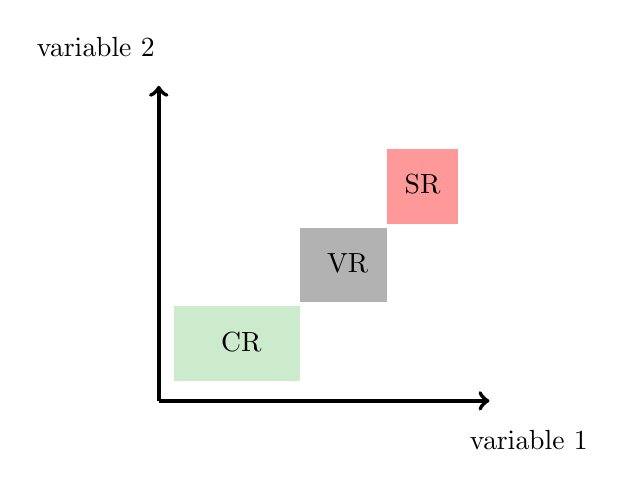
\begin{tikzpicture}
		\draw[line width =1.5pt,->] (0,0) -- (4.2,0);
		\node[](A) at (4.7,-0.5) {variable 1};
		\draw[line width =1.5pt,->] (0,0) -- (0,4.0);
		\node[](B) at (-0.8,4.5) {variable 2};
		\fill[green!60!black!20] (0.2,0.25) rectangle (1.8,1.2);
		\node[](E) at (1.05,0.75) {CR};
		\fill[gray!60] (1.8,1.25) rectangle (2.9,2.2);
%				\fill[gray!60] (1.8,1.25) rectangle (2.9,2.2);
		\node[](L) at (2.4,1.75) {VR};
		\fill[red!40] (2.9,2.25) rectangle (3.8,3.2);
		\node[](M) at (3.35,2.75) {SR};
		\end{tikzpicture}
		\caption{Visualisation of signal, control and validation regions and a typical arrangement in phase space \label{fig:stat:regions}}
\end{figure}



\section{Signal region optimisation}
\label{sec:analysis:sroptimisationSection}
In the following, a description of the optimisation procedure used to define the signal regions is given.
A grid of simulated signal events obtained by varying the masses of \None and \Cone / \Ntwo has been used to perform the signal region optimisation.
The overall signal mass point grid can be seen in Figure \ref{fig:analysis:grid}.
%This includes an extension of the available mass points towards higher \Mntwo masses,  which where not yet available at the optimisation stage of the analysis described below.  This extension is not impacting the sensitivity reach or signal region definition of the analysis.

\subsection{Choice of kinematic variables}
To understand the difference between a potential supersymmetric particle production compared to a \ac{SM} process,  various kinematic variables can be studied.  \\
%This can be properties of the reconstructed particles, such as the transverse momentum ($p_T$),  pseudorapidity ($\eta$) and azimuthal angle $\Phi$,  as well as kinematic variables constructed from these properties.
One of the kinematic variables of interest in a di-tau final state is the \textit{visible mass} of the di-tau system, $m_{vis}(\tau_1,\tau_2)$, constructed using the four-momenta of the two leading tau candidates in the event.  This variable only takes into account the visible components of the hadronic decaying tau, therefore not considering the missing momentum carried by the tau neutrinos.

%In the case of a particle's decay product being invisible to the ATLAS detector,  a part of the momentum will be missing,  shifting the particle's invariant mass calculation.
To account for the invisible decay products,  the missing transverse momentum can be included in an adapted "invisible" mass, the transverse mass $m_T$:

\begin{align}
\label{eq:sr_optimisation:mt} m_T = \sqrt{2p_T^{\ell}E_T^{\text{miss}}(1-\cos(\Delta \phi(\vec{\ell},\vec{p}_T^{\text{miss}}))}
\end{align}

For example,  in the case of a leptonic W-bosons decay, the $m_T$ shows an endpoint at the mass of the W boson. \\
In the case of two hadronically decaying tau leptons,  the sum of the transverse masses $m_{Tsum}$ can be powerful in discriminating \ac{SM} background from signal:

\begin{align}
\label{eq:sr_optimisation:mtsum} m_{Tsum} = m_T(\tau_1)+m_T(\tau_2)
\end{align}

With $m_T(\tau_1)$ denoting the transverse mass as defined in equation \eqref{eq:sr_optimisation:mt} with the lepton as the leading,  highest momentum, hadronic decaying tau lepton. 
The transverse mass concept can be extended to pair produced particles partially decaying into invisible particles, using the definition by Barr, Lester,  Stephens and Summers \cite{mt2original, mt2discussion} of the stransverse mass:

\begin{align}
m_{T2} ( \textbf{p}_T^{\ell_1}, \textbf{p}_T^{\ell_2}, \textbf{p}_T^{\text{miss}}) \equiv  \underset{\textbf{p}_1^\text{miss} + \textbf{p}_2^\text{miss} = \textbf{p}_T^\text{miss}}{\text{min}} \left[ \text{max} \{ m_T(\textbf{p}_T^{\ell_1}, \textbf{p}_1^{\text{miss}}),   m_T(\textbf{p}_T^{\ell_2}, \textbf{p}_2^{\text{miss}}) \} \right]
\end{align}

Here the momentum ($\textbf{p}_T^{\ell_1}, \textbf{p}_T^{\ell_2}$) of the two leptons in the event (for example the visible part of the hadronic tau decay) are combined into a transverse mass with parts of the missing transverse momentum, split into $\textbf{p}_1^\text{miss}$ and $\textbf{p}_2^\text{miss}$.  
This variable shows an endpoint at the mass of the pair-produced particle,  leading to a usually lower end-point of the distribution for \ac{SM} background processes in comparison to the \ac{SUSY} model considered. The mass of the invisible particles is assumed to be zero.

If an event includes more than two leptons (with a maximum number of leptons $n_\ell$),  it can be useful to perform a maximisation over the $m_{T2}$ values resulting from all possible lepton pairs:

\begin{align}
m_{T2}^\text{max} = \max_{\substack{i = 1,...,n_\ell \\ j = 2,..., n_\ell \\ i \neq j}} \left[ m_{T2}(\textbf{p}_T^{\ell_i}, \textbf{p}_T^ {\ell_j},\textbf{p}_T^{\text{miss}}) \right] \label{eq:sr_optimisation:mt2max}
\end{align}

\FloatBarrier
\subsection{SR optimisation procedure}
As starting point of the optimisation,  the kinematic variables described in the previous section are studied for \ac{SM} background events and signal events. In the following plots, all \ac{SM} background distributions shown are obtained from Monte Carlo.
In Figure \ref{fig:app:LMpreselections}, some kinematic variables are shown after the selection with an asymmetric di-tau trigger selection as well as a b-jet veto and light lepton veto.  %These preselections are used to gauge the discriminating power of a set of kinematic variables for varying signal mass points.
A selection of signal points is used to gauge the effectiveness of the variables to isolate a signal.
In Figure \ref{fig:analysis:opt:mt2max},  $m_{T2}^\text{max}$,  as defined in \eqref{eq:sr_optimisation:mt2max} can be compared with Figure \ref{fig:analysis:opt:mt2},  showing $m_{T2}$. The maximisation over all tau pairs in the event leads to a slight improvement in sensitivity compared to $m_{T2}$ calculated using the two leading tau candidates.  In the lower panels of Figure \ref{fig:app:LMpreselections},  a simplified sensitivity measure $Z_n$ \cite{zndefinition} including a 30\% flat systematic uncertainty is used to gauge the sensitivity of each variable to the signal model.  A $Z_n$ implementation of the RooStats \cite{RooStats} package within the ROOT \cite{Root} software framework is used.  This sensitivity measure is used to estimate the signal to background separation power as fully estimated with hypothesis testing as described in section \ref{sec:analysis:stats}.
As can be seen in Figures \ref{fig:analysis:opt:mttau1} and Fig.  \ref{fig:analysis:opt:mttau2} in comparison to the sum of both $m_T$ shown in Figure \ref{fig:analysis:opt:summt},  summing the transverse mass of the two leading taus offers a slightly higher discriminating power than the single transverse masses.
%/mnt/lustre/projects/epp/general/atlas/dk352/C1N2_tau/plotting_kinematics/19v02plotting/April20/210420_optimising

\begin{figure}[htpb]
\centering
\subfloat[$m_{T2}^\text{max}$ \label{fig:analysis:opt:mt2max} ]{\includegraphics[width=0.49\textwidth]{figures/SignalOp_Thesis_260722_AG_noATLAS/asymbasicLLV_mt2maxSROpt.pdf}}
\subfloat[$m_{T2}$ \label{fig:analysis:opt:mt2}]{\includegraphics[width=0.49\textwidth]{figures/SignalOp_Thesis_260722_AG_noATLAS/asymbasicLLV_mt2SROpt.pdf}}\\
\subfloat[$m_T(\tau_1,E_T^\text{miss})$ \label{fig:analysis:opt:mttau1}]{\includegraphics[width=0.49\textwidth]{figures/SignalOp_Thesis_260722_AG_noATLAS/asymbasicLLV_Mt_Tau1metSROpt.pdf}}
\subfloat[$m_T(\tau_2,E_T^\text{miss})$ \label{fig:analysis:opt:mttau2}]{\includegraphics[width=0.49\textwidth]{figures/SignalOp_Thesis_260722_AG_noATLAS/asymbasicLLV_Mt_Tau2metSROpt.pdf}}\\
\subfloat[$m_{Tsum}$ \label{fig:analysis:opt:summt}]{\includegraphics[width=0.49\textwidth]{figures/SignalOp_Thesis_260722_AG_noATLAS/asymbasicLLV_SumMtTauSROpt.pdf}}
\subfloat[$m_{vis}(\tau_1,\tau_2)$ \label{fig:analysis:opt:mvis}]{\includegraphics[width=0.49\textwidth]{figures/SignalOp_Thesis_260722_AG_noATLAS/asymbasicLLV_mvisTauTauSROpt.pdf}}\\
\subfloat[$E_T^\text{miss}$ \label{fig:analysis:opt:met}]{\includegraphics[width=0.49\textwidth]{figures/SignalOp_Thesis_260722_AG_noATLAS/asymbasicLLV_metSROpt.pdf}}
%\subfloat[$meff$]{\includegraphics[width=0.45\textwidth]{figures/C1N2SS/SROptAppendix/asym_basicLLV_meff_mc16_a_e_d_.pdf}} \\
\subfloat[$\Delta\phi(\tau_1,\tau_2)$ \label{fig:analysis:opt:deltaphi}]{\includegraphics[width=0.49\textwidth]{figures/SignalOp_Thesis_260722_AG_noATLAS/asymbasicLLV_deltaPhiTauTauSROpt.pdf}}
%\subfloat[$\Delta\phi(\tau_1,E_T^\text{miss})$]{\includegraphics[width=0.45\textwidth]{figures/C1N2SS/SROptAppendix/asym_basicLLV_deltaPhiTau1Met_mc16_a_e_d_.pdf}}
\caption{Kinematic variable distributions for SS scenario after a loose preselection. Error bands include statistical uncertainties only.  The lower panel shows the significance $Z_n$ including a 30 \% systematic uncertainty assumption. 
\label{fig:app:LMpreselections}}
\end{figure}

%210420_improveSign

In case of a low m(\Cone,\Ntwo) (low mass scenario, SR-C1N2SS-LM),  a cut of $E_T^\text{miss} < 150 \text{ GeV}$ is introduced.  The case of high \Cone, \Ntwo mass (SR-C1N2SS-HM) is defined by $E_T^\text{miss}>~150 \text{ GeV}$. The effect of multiple cuts (not applied consecutively) on the overall sensitivity is given in Figure~\ref{fig:app:LMgridstudies}.



\begin{figure}[h]
\centering
\subfloat[$m_{T2}^\text{max} > 20 \text{ GeV} $]{\includegraphics[width=0.49\textwidth]{figures/C1N2SS/SROptAppendix_Improved/SignificancesTrueonlymt2_20.pdf}}
\subfloat[$m_{T2}^\text{max} > 50 \text{ GeV} $]{\includegraphics[width=0.49\textwidth]{figures/C1N2SS/SROptAppendix_Improved/SignificancesTrueonlymt2_50.pdf}} \\
\subfloat[$m_{Tsum} > 150 \text{ GeV}$]{\includegraphics[width=0.49\textwidth]{figures/C1N2SS/SROptAppendix_Improved/SignificancesTrueonlySumMt_150.pdf}}
\subfloat[$m_{Tsum} > 200 \text{ GeV}$]{\includegraphics[width=0.49\textwidth]{figures/C1N2SS/SROptAppendix_Improved/SignificancesTrueonlySumMt_200.pdf}}\\
\caption{ Significance estimation including a $30 \%$ flat systematic uncertainty.\label{fig:app:LMgridstudies}}
\end{figure}

An $m_{Tsum} > 200 \text{ GeV}$ selection was chosen because it gives a higher sensitivity toward the diagonal of the (\Cone/\Ntwo, \None) mass plane.
The additional requirement $\Delta\phi(\tau_1,\tau_2) > 1.5$ is included in the signal region definition,  to reduce the signal contamination when estimating the multi-jet background (see section \ref{sec:bkgestimation:ABCD}.
The optimisation for the high mass case followed a very similar approach, leading to the two orthogonal signal regions defined in Table~\ref{tab:SRdef}.
%This selection and an inversion of the transverse mass sum requirement offered the basis of the ABCD method,  allowing for a multi-jet estimation.  This is in detail described in section \ref{sec:bkgestimation:ABCD}.
%A preliminary estimation of the multi-jet background lead to the introduction of a $\Delta\phi(\tau_1,\tau_2)+\Delta\phi(\tau_1, E_T^\text{miss})>2.5$ cut to reduce the signal contamination within the ABCD regions.


%With a multi-jet background estimate included, multiple further cuts on kinematic variables have been tested according to their performance over the grid, with a particular focus on the sensitivitiy towards the kinematic diagonal (\Mnone close to \Mntwo). These include:
%\begin{itemize}
%\item $m_T(\tau_1)+m_T(\tau_2)$ > [240, 260, 280, 300,400,500]
%\item $m_{vis}(\tau_1,\tau_2) > 130$, $m_{vis}(\tau_1,\tau_2) > 400$, $m_{vis}(\tau_1,\tau_2) \in [130,400]$
%\item $E_T^\text{miss}$ > [50,60,70,80]
%\item $m_{T2}^\text{max}$ > [10,20,30,40,50,60,70,80]
%\item Number of signal jets < [2,3]
%\end{itemize}

%Multiple different combinations of these cuts have been taken into account and their effect considered singular as well as in combination. These iterative studies led to the definitions given in section \ref{sec:SR:SS}.

 %The sum of the leading taus transverse mass ($m_T(\tau_1)+m_T(\tau_2)$) was used to define ABCD regions and with that a signal region optimisation phase space, using a $m_T(\tau_1)+m_T(\tau_2) > 300 \text{GeV}$ requirement.

%%%%%%%%%%%%%%%%%%%%%%%%%%%%%%%%%%%%%%%%%%%%%%%%%%%%%%%%%%%%%%%%%%%%%%%%%%%%%%%%%%%


\begin{table}[htpb!]
\centering
\begin{tabular}{c|c} \hline
SR-C1N2SS-LM & SR-C1N2SS-HM \\ \hline \hline
\multicolumn{2}{c}{$>=$ 2 medium taus (SS) } \\
\multicolumn{2}{c}{$b$-jet veto} \\
$\Delta\Phi(\tau_1,\tau_2)  > 1.5 $&-\\
${N}_{jets} <$3 & - \\ \hline
$m_{Tsum}  > 200 \text{ GeV} $ & $m_{Tsum} > 450 \text{ GeV}$\\
\multicolumn{2}{c}{$ m_{T2}^{\text{max}} > 80 \text{ GeV}$  } \\\hline %\vspace{0.5cm}\\ \hline %\vspace{1cm}
 asymmetric di-tau trigger  & di-tau+\met trigger \\
$\met <$ 150 GeV    & $\met >$ 150 GeV          \\
\multicolumn{2}{c}{$\tau_{1}$ and $\tau_{2}$ $p_\text{T}$ requirements described in Table
  \ref{tab:analysis:trigger} in Section \ref{sec:analysis:eventselection}}\\
\hline
\end{tabular}
\caption{Summary of selection requirements for the signal regions.
\label{tab:SRdef} }
\end{table}

An overview of the event yields in both signal regions is shown in table \ref{tab:SS:SRyields}. All backgrounds apart from the Multi-jet background are taken from MC simulation with only statistical uncertainties included below.  The Multijet estimation is performed using a data-driven method,  discussed in detail in section \ref{sec:bkgestimation:ABCD}.

\begin{table}
\centering
% Preview source code for paragraph 0

\begin{tabular}{c|c|c}
\hline
SM-process & SR-C1N2SS-LM & SR-C1N2SS-HM\tabularnewline
\hline
\hline
%\hline
Top & $0.01\pm0.01$ & $0.84\pm0.36$\tabularnewline
%\hline
Multi-boson & $0.47\pm0.11$ & $0.81\pm0.21$\tabularnewline
%\hline
Multi-jet & $0.94\pm0.27$ & $ -0.086 \pm 0.31$\tabularnewline
%\hline
$W$+jets & $0.32\pm0.32$ & $0.10\pm0.10$\tabularnewline
%\hline
$Z$+jets & $0.20\pm0.20$ & $0.59\pm0.56$\tabularnewline
%\hline
Higgs & $0.00\pm0.00$ & $0.02\pm0.00$\tabularnewline
\hline
%\hline
SM total & $1.95 \pm 0.48$ & $2.35\pm0.80$\tabularnewline
%\hline
\hline
%Ref. point (325, 175) & $18.20\pm3.00$ & $2.91\pm0.51$\tabularnewline
Ref. point (325, 175) & $ 7.80 \pm 1.27 $& $ 2.26 \pm 0.71 $\tabularnewline
%\hline
%Ref. point (500, 300)  & $5.25\pm0.75$ & $4.68\pm10.78$\tabularnewline
Ref. point (500, 300)  & $ 3.78 \pm 0.65 $& $ 5.62 \pm 0.88 $\tabularnewline
%\hline
%Ref. point (900, 300) & $0.71\pm0.07$ & $6.37\pm0.21$\tabularnewline
Ref. point (900, 300) &  $ 0.84 \pm 0.07 $ & $ 6.23 \pm 0.21 $\tabularnewline
\hline
\end{tabular}
\caption{Number of events in the signal regions for SM backgrounds, including statistical
  uncertainties.  The SM MC backgrounds are normalised to 139~\ifb. The multi-jet contribution is estimated
  from data with a simplified ABCD method described in Section
  \ref{sec:bkgestimation:ABCD}. Only statistical uncertainty are considered for MC
  estimated processes and multi-jet.
%The proper results are showed in Table~\ref{ysr0} in Section \ref{sec:results-bkgfit}.
\label{tab:SS:SRyields}}
\end{table}

%%%%%%%%%%%%%%%%%%%%%%%%%%%%%%%%%%%%%%%%%%%%%%%%%%%%%%%%%%%%%%%%%%%%%%%%%%%%%%%%%%%
%%%%    N-1 plots
%%%%%%%%%%%%%%%%%%%%%%%%%%%%%%%%%%%%%%%%%%%%%%%%%%%%%%%%%%%%%%%%%%%%%%%%%%%%%%%%%%%

Kinematic distributions in the signal regions, with requirements on the shown variable removed ("N-1 distributions"), can be seen in figure \ref{fig:SS:SRlowmass} for SR-C1N2SS-LM,  and figure \ref{fig:SS:SRhighmass} for SR-C1N2SS-HM,  already including the multi-jet estimation as well as systematic uncertainties discussed in section \ref{sec:analysis:bkgestimation} and \ref{sec:analysis:systematics}, respectively. 

\begin{figure}[!htpb]
\centering
  \subfloat[$\Delta\Phi(\tau_1,\tau_2)$]{\includegraphics[width=0.49\textwidth]{figures/UpdatedThesisFigures_noATLAS/LowMass/DeltaPhi_N1_improved.pdf}}
  \subfloat[${N}_{jets} $]{\includegraphics[width=0.49\textwidth]{figures/UpdatedThesisFigures_noATLAS/LowMass/SigJets_N1_improved.pdf}}\\
  \subfloat[$ m_{T2}^{\text{max}} $]{\includegraphics[width=0.49\textwidth]{figures/UpdatedThesisFigures_noATLAS/LowMass/Mt2_N1_improved.pdf}}
  \caption{``N-1'' distributions of relevant kinematic variables after SR-C1N2SS-LM requirements, except the one on the
shown variable, have been applied.
The stacked histograms show the expected SM backgrounds estimated from \ac{MC}, normalised to 139~\ifb as well as Multi-jet expectation as described in section \ref{sec:bkgestimation:ABCD}.
\label{fig:SS:SRlowmass}Statistical uncertainties and systematic uncertainties as discussed in section \ref{sec:analysis:systematics} are included in the error band. }
\end{figure}

\begin{figure}[!htpb]
\centering
\subfloat[$m_{Tsum}$]{\includegraphics[width=0.49\textwidth]{figures/UpdatedThesisFigures_noATLAS/HighMass/SumMt_N1_improved.pdf}}
\subfloat[$ m_{T2}^{\text{max}} $]{\includegraphics[width=0.49\textwidth]{figures/UpdatedThesisFigures_noATLAS/HighMass/Mt2_N1_improved.pdf}}
  \caption{``N-1'' distributions of relevant kinematic variables after SR-C1N2SS-HM requirements, except the one on the
shown variable, have been applied. The stacked histograms show the expected \ac{SM} backgrounds estimated from \ac{MC}, normalised to 139 ~\ifb as well as Multi-jet expectation as described in section \ref{sec:bkgestimation:ABCD}. Statistical and systematic uncertainties as discussed in \ref{sec:analysis:systematics} are included in the error band. 
\label{fig:SS:SRhighmass} }
\end{figure}

Further kinematic distribution in both signal regions can be seen in \ref{fig:SS:SRlowDistr} and \ref{fig:SS:SRhighDistr}, respectively. This clearly shows that no further requirements on other kinematic variables are able to gain in sensitivity,  at least not while allowing for sufficient remaining statistics in the \ac{SM} background simulations.

\begin{figure}[!htpb]
\centering
\subfloat[]{\includegraphics[width=0.49\textwidth]{figures/UpdatedThesisFigures_noATLAS/LowMass/asymSRD_wDPhiOnly_TRIALsummt200_mvis_nomvisup_MT280_deltaphi_signaljets2_noLLV_nomvis_deltaPhiTau1MetSRL.pdf}}
\subfloat[]{\includegraphics[width=0.49\textwidth]{figures/UpdatedThesisFigures_noATLAS/LowMass/asymSRD_wDPhiOnly_TRIALsummt200_mvis_nomvisup_MT280_deltaphi_signaljets2_noLLV_nomvis_deltaR_etaSRL.pdf}}\\
\subfloat[]{\includegraphics[width=0.49\textwidth]{figures/UpdatedThesisFigures_noATLAS/LowMass/asymSRD_wDPhiOnly_TRIALsummt200_mvis_nomvisup_MT280_deltaphi_signaljets2_noLLV_nomvis_metSRL.pdf}}
\subfloat[]{\includegraphics[width=0.49\textwidth]{figures/UpdatedThesisFigures_noATLAS/LowMass/asymSRD_wDPhiOnly_TRIALsummt200_mvis_nomvisup_MT280_deltaphi_signaljets2_noLLV_nomvis_tau1PtSRL.pdf}}\\
\subfloat[]{\includegraphics[width=0.49\textwidth]{figures/UpdatedThesisFigures_noATLAS/LowMass/asymSRD_wDPhiOnly_TRIALsummt200_mvis_nomvisup_MT280_deltaphi_signaljets2_noLLV_nomvis_tau2PtSRH.pdf}}
\subfloat[]{\includegraphics[width=0.49\textwidth]{figures/UpdatedThesisFigures_noATLAS/LowMass/asymSRD_wDPhiOnly_TRIALsummt200_mvis_nomvisup_MT280_deltaphi_signaljets2_noLLV_nomvis_mvisTauTauSRL.pdf}}
  \caption{Remaining kinematic distributions in SR-C1N2SS-LM, for all variables not used in the signal region definition.  The error band includes statistical and systematic uncertainties. The lower panel shows the significance $Z_n$ including a 30 \% systematic uncertainty assumption. 
\label{fig:SS:SRlowDistr}}.
\end{figure}

\begin{figure}[!htpb]
\centering
  \subfloat[]{\includegraphics[width=0.49\textwidth]{figures//UpdatedThesisFigures_noATLAS/HighMass/ditauMETSRSummthighmt2_deltaEtaTauTau.pdf} }
  \subfloat[]{\includegraphics[width=0.49\textwidth]{figures//UpdatedThesisFigures_noATLAS/HighMass/ditauMETSRSummthighmt2_deltaPhiTau1MetSRL.pdf} }\\
  \subfloat[]{\includegraphics[width=0.49\textwidth]{figures//UpdatedThesisFigures_noATLAS/HighMass/ditauMETSRSummthighmt2_deltaPhiTauTauSRH.pdf} }
     \subfloat[]{\includegraphics[width=0.49\textwidth]{figures//UpdatedThesisFigures_noATLAS/HighMass/ditauMETSRSummthighmt2_deltaR_etaSRL.pdf} }\\
  \subfloat[]{\includegraphics[width=0.49\textwidth]{figures/UpdatedThesisFigures_noATLAS/HighMass/ditauMETSRSummthighmt2_metSRH.pdf} }
  \subfloat[]{\includegraphics[width=0.49\textwidth]{figures/UpdatedThesisFigures_noATLAS/HighMass/ditauMETSRSummthighmt2_mvisTauTauSRH.pdf} }
  \caption{Remaining kinematic distributions in SR-C1N2SS-HM, for all variables not used in the signal region definition. The error band includes statistical and systematic uncertainties. The lower panel shows the significance $Z_n$ including a 30 \% systematic uncertainty assumption. 
\label{fig:SS:SRhighDistr}}
\end{figure}


%%%%%%%%%%%%%%%%%%%%%%%%%%%%%%%%%%%%%%%%%%%%%%%%%%%%%%%%%%%%%%%%%%%%%%%%%%%%%%%%%%%
%%%% sensitivity
%%%%%%%%%%%%%%%%%%%%%%%%%%%%%%%%%%%%%%%%%%%%%%%%%%%%%%%%%%%%%%%%%%%%%%%%%%%%%%%%%%%
 The estimated sensitivity of both signal regions, using the significance measure $Z_n$ is shown in figure \ref{fig:SS:SRsign}. This is a first estimate of the sensitivity of these regions to the gaugino pair production under investigation.

\begin{figure}[!htpb]
\centering
  \subfloat[SR-C1N2SS-LM]{\includegraphics[width=0.49\textwidth]{figures/C1N2SS/SRdefs/LowMass/SRLowMassSign_improved.pdf}}
  \subfloat[SR-C1N2SS-HM]{\includegraphics[width=0.49\textwidth]{figures/C1N2SS/SRdefs/HighMass/SRHighMassSign_improved.pdf}}
  \caption{Significance distribution for the (a) SR-C1N2SS-LM, (b)
  SR-C1N2SS-HM for 139~\ifb. The statistical uncertainty
 and 30\% systematic uncertainty on SM backgrounds are included in the $\text{Z}_{\text{N}}$
calculation. 
\label{fig:SS:SRsign}}
\end{figure}

\label{sec:analysis:sroptimisation}

%In the following, a description of the optimisation procedure used to define the signal regions is given.
A grid of simulated signal events obtained by varying the masses of \None and \Cone / \Ntwo has been used to perform the signal region optimisation.
The overall signal mass point grid can be seen in Figure \ref{fig:analysis:grid}.
%This includes an extension of the available mass points towards higher \Mntwo masses,  which where not yet available at the optimisation stage of the analysis described below.  This extension is not impacting the sensitivity reach or signal region definition of the analysis.

\subsection{Choice of kinematic variables}
To understand the difference between a potential supersymmetric particle production compared to a \ac{SM} process,  various kinematic variables can be studied.  \\
%This can be properties of the reconstructed particles, such as the transverse momentum ($p_T$),  pseudorapidity ($\eta$) and azimuthal angle $\Phi$,  as well as kinematic variables constructed from these properties.
One of the kinematic variables of interest in a di-tau final state is the \textit{visible mass} of the di-tau system, $m_{vis}(\tau_1,\tau_2)$, constructed using the four-momenta of the two leading tau candidates in the event.  This variable only takes into account the visible components of the hadronic decaying tau, therefore not considering the missing momentum carried by the tau neutrinos.

%In the case of a particle's decay product being invisible to the ATLAS detector,  a part of the momentum will be missing,  shifting the particle's invariant mass calculation.
To account for the invisible decay products,  the missing transverse momentum can be included in an adapted "invisible" mass, the transverse mass $m_T$:

\begin{align}
\label{eq:sr_optimisation:mt} m_T = \sqrt{2p_T^{\ell}E_T^{\text{miss}}(1-\cos(\Delta \phi(\vec{\ell},\vec{p}_T^{\text{miss}}))}
\end{align}

For example,  in the case of a leptonic W-bosons decay, the $m_T$ shows an endpoint at the mass of the W boson. \\
In the case of two hadronically decaying tau leptons,  the sum of the transverse masses $m_{Tsum}$ can be powerful in discriminating \ac{SM} background from signal:

\begin{align}
\label{eq:sr_optimisation:mtsum} m_{Tsum} = m_T(\tau_1)+m_T(\tau_2)
\end{align}

With $m_T(\tau_1)$ denoting the transverse mass as defined in equation \eqref{eq:sr_optimisation:mt} with the lepton as the leading,  highest momentum, hadronic decaying tau lepton. 
The transverse mass concept can be extended to pair produced particles partially decaying into invisible particles, using the definition by Barr, Lester,  Stephens and Summers \cite{mt2original, mt2discussion} of the stransverse mass:

\begin{align}
m_{T2} ( \textbf{p}_T^{\ell_1}, \textbf{p}_T^{\ell_2}, \textbf{p}_T^{\text{miss}}) \equiv  \underset{\textbf{p}_1^\text{miss} + \textbf{p}_2^\text{miss} = \textbf{p}_T^\text{miss}}{\text{min}} \left[ \text{max} \{ m_T(\textbf{p}_T^{\ell_1}, \textbf{p}_1^{\text{miss}}),   m_T(\textbf{p}_T^{\ell_2}, \textbf{p}_2^{\text{miss}}) \} \right]
\end{align}

Here the momentum ($\textbf{p}_T^{\ell_1}, \textbf{p}_T^{\ell_2}$) of the two leptons in the event (for example the visible part of the hadronic tau decay) are combined into a transverse mass with parts of the missing transverse momentum, split into $\textbf{p}_1^\text{miss}$ and $\textbf{p}_2^\text{miss}$.  
This variable shows an endpoint at the mass of the pair-produced particle,  leading to a usually lower end-point of the distribution for \ac{SM} background processes in comparison to the \ac{SUSY} model considered. The mass of the invisible particles is assumed to be zero.

If an event includes more than two leptons (with a maximum number of leptons $n_\ell$),  it can be useful to perform a maximisation over the $m_{T2}$ values resulting from all possible lepton pairs:

\begin{align}
m_{T2}^\text{max} = \max_{\substack{i = 1,...,n_\ell \\ j = 2,..., n_\ell \\ i \neq j}} \left[ m_{T2}(\textbf{p}_T^{\ell_i}, \textbf{p}_T^ {\ell_j},\textbf{p}_T^{\text{miss}}) \right] \label{eq:sr_optimisation:mt2max}
\end{align}

\FloatBarrier
\subsection{SR optimisation procedure}
As starting point of the optimisation,  the kinematic variables described in the previous section are studied for \ac{SM} background events and signal events. In the following plots, all \ac{SM} background distributions shown are obtained from Monte Carlo.
In Figure \ref{fig:app:LMpreselections}, some kinematic variables are shown after the selection with an asymmetric di-tau trigger selection as well as a b-jet veto and light lepton veto.  %These preselections are used to gauge the discriminating power of a set of kinematic variables for varying signal mass points.
A selection of signal points is used to gauge the effectiveness of the variables to isolate a signal.
In Figure \ref{fig:analysis:opt:mt2max},  $m_{T2}^\text{max}$,  as defined in \eqref{eq:sr_optimisation:mt2max} can be compared with Figure \ref{fig:analysis:opt:mt2},  showing $m_{T2}$. The maximisation over all tau pairs in the event leads to a slight improvement in sensitivity compared to $m_{T2}$ calculated using the two leading tau candidates.  In the lower panels of Figure \ref{fig:app:LMpreselections},  a simplified sensitivity measure $Z_n$ \cite{zndefinition} including a 30\% flat systematic uncertainty is used to gauge the sensitivity of each variable to the signal model.  A $Z_n$ implementation of the RooStats \cite{RooStats} package within the ROOT \cite{Root} software framework is used.  This sensitivity measure is used to estimate the signal to background separation power as fully estimated with hypothesis testing as described in section \ref{sec:analysis:stats}.
As can be seen in Figures \ref{fig:analysis:opt:mttau1} and Fig.  \ref{fig:analysis:opt:mttau2} in comparison to the sum of both $m_T$ shown in Figure \ref{fig:analysis:opt:summt},  summing the transverse mass of the two leading taus offers a slightly higher discriminating power than the single transverse masses.
%/mnt/lustre/projects/epp/general/atlas/dk352/C1N2_tau/plotting_kinematics/19v02plotting/April20/210420_optimising

\begin{figure}[htpb]
\centering
\subfloat[$m_{T2}^\text{max}$ \label{fig:analysis:opt:mt2max} ]{\includegraphics[width=0.49\textwidth]{figures/SignalOp_Thesis_260722_AG_noATLAS/asymbasicLLV_mt2maxSROpt.pdf}}
\subfloat[$m_{T2}$ \label{fig:analysis:opt:mt2}]{\includegraphics[width=0.49\textwidth]{figures/SignalOp_Thesis_260722_AG_noATLAS/asymbasicLLV_mt2SROpt.pdf}}\\
\subfloat[$m_T(\tau_1,E_T^\text{miss})$ \label{fig:analysis:opt:mttau1}]{\includegraphics[width=0.49\textwidth]{figures/SignalOp_Thesis_260722_AG_noATLAS/asymbasicLLV_Mt_Tau1metSROpt.pdf}}
\subfloat[$m_T(\tau_2,E_T^\text{miss})$ \label{fig:analysis:opt:mttau2}]{\includegraphics[width=0.49\textwidth]{figures/SignalOp_Thesis_260722_AG_noATLAS/asymbasicLLV_Mt_Tau2metSROpt.pdf}}\\
\subfloat[$m_{Tsum}$ \label{fig:analysis:opt:summt}]{\includegraphics[width=0.49\textwidth]{figures/SignalOp_Thesis_260722_AG_noATLAS/asymbasicLLV_SumMtTauSROpt.pdf}}
\subfloat[$m_{vis}(\tau_1,\tau_2)$ \label{fig:analysis:opt:mvis}]{\includegraphics[width=0.49\textwidth]{figures/SignalOp_Thesis_260722_AG_noATLAS/asymbasicLLV_mvisTauTauSROpt.pdf}}\\
\subfloat[$E_T^\text{miss}$ \label{fig:analysis:opt:met}]{\includegraphics[width=0.49\textwidth]{figures/SignalOp_Thesis_260722_AG_noATLAS/asymbasicLLV_metSROpt.pdf}}
%\subfloat[$meff$]{\includegraphics[width=0.45\textwidth]{figures/C1N2SS/SROptAppendix/asym_basicLLV_meff_mc16_a_e_d_.pdf}} \\
\subfloat[$\Delta\phi(\tau_1,\tau_2)$ \label{fig:analysis:opt:deltaphi}]{\includegraphics[width=0.49\textwidth]{figures/SignalOp_Thesis_260722_AG_noATLAS/asymbasicLLV_deltaPhiTauTauSROpt.pdf}}
%\subfloat[$\Delta\phi(\tau_1,E_T^\text{miss})$]{\includegraphics[width=0.45\textwidth]{figures/C1N2SS/SROptAppendix/asym_basicLLV_deltaPhiTau1Met_mc16_a_e_d_.pdf}}
\caption{Kinematic variable distributions for SS scenario after a loose preselection. Error bands include statistical uncertainties only.  The lower panel shows the significance $Z_n$ including a 30 \% systematic uncertainty assumption. 
\label{fig:app:LMpreselections}}
\end{figure}

%210420_improveSign

In case of a low m(\Cone,\Ntwo) (low mass scenario, SR-C1N2SS-LM),  a cut of $E_T^\text{miss} < 150 \text{ GeV}$ is introduced.  The case of high \Cone, \Ntwo mass (SR-C1N2SS-HM) is defined by $E_T^\text{miss}>~150 \text{ GeV}$. The effect of multiple cuts (not applied consecutively) on the overall sensitivity is given in Figure~\ref{fig:app:LMgridstudies}.



\begin{figure}[h]
\centering
\subfloat[$m_{T2}^\text{max} > 20 \text{ GeV} $]{\includegraphics[width=0.49\textwidth]{figures/C1N2SS/SROptAppendix_Improved/SignificancesTrueonlymt2_20.pdf}}
\subfloat[$m_{T2}^\text{max} > 50 \text{ GeV} $]{\includegraphics[width=0.49\textwidth]{figures/C1N2SS/SROptAppendix_Improved/SignificancesTrueonlymt2_50.pdf}} \\
\subfloat[$m_{Tsum} > 150 \text{ GeV}$]{\includegraphics[width=0.49\textwidth]{figures/C1N2SS/SROptAppendix_Improved/SignificancesTrueonlySumMt_150.pdf}}
\subfloat[$m_{Tsum} > 200 \text{ GeV}$]{\includegraphics[width=0.49\textwidth]{figures/C1N2SS/SROptAppendix_Improved/SignificancesTrueonlySumMt_200.pdf}}\\
\caption{ Significance estimation including a $30 \%$ flat systematic uncertainty.\label{fig:app:LMgridstudies}}
\end{figure}

An $m_{Tsum} > 200 \text{ GeV}$ selection was chosen because it gives a higher sensitivity toward the diagonal of the (\Cone/\Ntwo, \None) mass plane.
The additional requirement $\Delta\phi(\tau_1,\tau_2) > 1.5$ is included in the signal region definition,  to reduce the signal contamination when estimating the multi-jet background (see section \ref{sec:bkgestimation:ABCD}.
The optimisation for the high mass case followed a very similar approach, leading to the two orthogonal signal regions defined in Table~\ref{tab:SRdef}.
%This selection and an inversion of the transverse mass sum requirement offered the basis of the ABCD method,  allowing for a multi-jet estimation.  This is in detail described in section \ref{sec:bkgestimation:ABCD}.
%A preliminary estimation of the multi-jet background lead to the introduction of a $\Delta\phi(\tau_1,\tau_2)+\Delta\phi(\tau_1, E_T^\text{miss})>2.5$ cut to reduce the signal contamination within the ABCD regions.


%With a multi-jet background estimate included, multiple further cuts on kinematic variables have been tested according to their performance over the grid, with a particular focus on the sensitivitiy towards the kinematic diagonal (\Mnone close to \Mntwo). These include:
%\begin{itemize}
%\item $m_T(\tau_1)+m_T(\tau_2)$ > [240, 260, 280, 300,400,500]
%\item $m_{vis}(\tau_1,\tau_2) > 130$, $m_{vis}(\tau_1,\tau_2) > 400$, $m_{vis}(\tau_1,\tau_2) \in [130,400]$
%\item $E_T^\text{miss}$ > [50,60,70,80]
%\item $m_{T2}^\text{max}$ > [10,20,30,40,50,60,70,80]
%\item Number of signal jets < [2,3]
%\end{itemize}

%Multiple different combinations of these cuts have been taken into account and their effect considered singular as well as in combination. These iterative studies led to the definitions given in section \ref{sec:SR:SS}.

 %The sum of the leading taus transverse mass ($m_T(\tau_1)+m_T(\tau_2)$) was used to define ABCD regions and with that a signal region optimisation phase space, using a $m_T(\tau_1)+m_T(\tau_2) > 300 \text{GeV}$ requirement.

%%%%%%%%%%%%%%%%%%%%%%%%%%%%%%%%%%%%%%%%%%%%%%%%%%%%%%%%%%%%%%%%%%%%%%%%%%%%%%%%%%%


\begin{table}[htpb!]
\centering
\begin{tabular}{c|c} \hline
SR-C1N2SS-LM & SR-C1N2SS-HM \\ \hline \hline
\multicolumn{2}{c}{$>=$ 2 medium taus (SS) } \\
\multicolumn{2}{c}{$b$-jet veto} \\
$\Delta\Phi(\tau_1,\tau_2)  > 1.5 $&-\\
${N}_{jets} <$3 & - \\ \hline
$m_{Tsum}  > 200 \text{ GeV} $ & $m_{Tsum} > 450 \text{ GeV}$\\
\multicolumn{2}{c}{$ m_{T2}^{\text{max}} > 80 \text{ GeV}$  } \\\hline %\vspace{0.5cm}\\ \hline %\vspace{1cm}
 asymmetric di-tau trigger  & di-tau+\met trigger \\
$\met <$ 150 GeV    & $\met >$ 150 GeV          \\
\multicolumn{2}{c}{$\tau_{1}$ and $\tau_{2}$ $p_\text{T}$ requirements described in Table
  \ref{tab:analysis:trigger} in Section \ref{sec:analysis:eventselection}}\\
\hline
\end{tabular}
\caption{Summary of selection requirements for the signal regions.
\label{tab:SRdef} }
\end{table}

An overview of the event yields in both signal regions is shown in table \ref{tab:SS:SRyields}. All backgrounds apart from the Multi-jet background are taken from MC simulation with only statistical uncertainties included below.  The Multijet estimation is performed using a data-driven method,  discussed in detail in section \ref{sec:bkgestimation:ABCD}.

\begin{table}
\centering
% Preview source code for paragraph 0

\begin{tabular}{c|c|c}
\hline
SM-process & SR-C1N2SS-LM & SR-C1N2SS-HM\tabularnewline
\hline
\hline
%\hline
Top & $0.01\pm0.01$ & $0.84\pm0.36$\tabularnewline
%\hline
Multi-boson & $0.47\pm0.11$ & $0.81\pm0.21$\tabularnewline
%\hline
Multi-jet & $0.94\pm0.27$ & $ -0.086 \pm 0.31$\tabularnewline
%\hline
$W$+jets & $0.32\pm0.32$ & $0.10\pm0.10$\tabularnewline
%\hline
$Z$+jets & $0.20\pm0.20$ & $0.59\pm0.56$\tabularnewline
%\hline
Higgs & $0.00\pm0.00$ & $0.02\pm0.00$\tabularnewline
\hline
%\hline
SM total & $1.95 \pm 0.48$ & $2.35\pm0.80$\tabularnewline
%\hline
\hline
%Ref. point (325, 175) & $18.20\pm3.00$ & $2.91\pm0.51$\tabularnewline
Ref. point (325, 175) & $ 7.80 \pm 1.27 $& $ 2.26 \pm 0.71 $\tabularnewline
%\hline
%Ref. point (500, 300)  & $5.25\pm0.75$ & $4.68\pm10.78$\tabularnewline
Ref. point (500, 300)  & $ 3.78 \pm 0.65 $& $ 5.62 \pm 0.88 $\tabularnewline
%\hline
%Ref. point (900, 300) & $0.71\pm0.07$ & $6.37\pm0.21$\tabularnewline
Ref. point (900, 300) &  $ 0.84 \pm 0.07 $ & $ 6.23 \pm 0.21 $\tabularnewline
\hline
\end{tabular}
\caption{Number of events in the signal regions for SM backgrounds, including statistical
  uncertainties.  The SM MC backgrounds are normalised to 139~\ifb. The multi-jet contribution is estimated
  from data with a simplified ABCD method described in Section
  \ref{sec:bkgestimation:ABCD}. Only statistical uncertainty are considered for MC
  estimated processes and multi-jet.
%The proper results are showed in Table~\ref{ysr0} in Section \ref{sec:results-bkgfit}.
\label{tab:SS:SRyields}}
\end{table}

%%%%%%%%%%%%%%%%%%%%%%%%%%%%%%%%%%%%%%%%%%%%%%%%%%%%%%%%%%%%%%%%%%%%%%%%%%%%%%%%%%%
%%%%    N-1 plots
%%%%%%%%%%%%%%%%%%%%%%%%%%%%%%%%%%%%%%%%%%%%%%%%%%%%%%%%%%%%%%%%%%%%%%%%%%%%%%%%%%%

Kinematic distributions in the signal regions, with requirements on the shown variable removed ("N-1 distributions"), can be seen in figure \ref{fig:SS:SRlowmass} for SR-C1N2SS-LM,  and figure \ref{fig:SS:SRhighmass} for SR-C1N2SS-HM,  already including the multi-jet estimation as well as systematic uncertainties discussed in section \ref{sec:analysis:bkgestimation} and \ref{sec:analysis:systematics}, respectively. 

\begin{figure}[!htpb]
\centering
  \subfloat[$\Delta\Phi(\tau_1,\tau_2)$]{\includegraphics[width=0.49\textwidth]{figures/UpdatedThesisFigures_noATLAS/LowMass/DeltaPhi_N1_improved.pdf}}
  \subfloat[${N}_{jets} $]{\includegraphics[width=0.49\textwidth]{figures/UpdatedThesisFigures_noATLAS/LowMass/SigJets_N1_improved.pdf}}\\
  \subfloat[$ m_{T2}^{\text{max}} $]{\includegraphics[width=0.49\textwidth]{figures/UpdatedThesisFigures_noATLAS/LowMass/Mt2_N1_improved.pdf}}
  \caption{``N-1'' distributions of relevant kinematic variables after SR-C1N2SS-LM requirements, except the one on the
shown variable, have been applied.
The stacked histograms show the expected SM backgrounds estimated from \ac{MC}, normalised to 139~\ifb as well as Multi-jet expectation as described in section \ref{sec:bkgestimation:ABCD}.
\label{fig:SS:SRlowmass}Statistical uncertainties and systematic uncertainties as discussed in section \ref{sec:analysis:systematics} are included in the error band. }
\end{figure}

\begin{figure}[!htpb]
\centering
\subfloat[$m_{Tsum}$]{\includegraphics[width=0.49\textwidth]{figures/UpdatedThesisFigures_noATLAS/HighMass/SumMt_N1_improved.pdf}}
\subfloat[$ m_{T2}^{\text{max}} $]{\includegraphics[width=0.49\textwidth]{figures/UpdatedThesisFigures_noATLAS/HighMass/Mt2_N1_improved.pdf}}
  \caption{``N-1'' distributions of relevant kinematic variables after SR-C1N2SS-HM requirements, except the one on the
shown variable, have been applied. The stacked histograms show the expected \ac{SM} backgrounds estimated from \ac{MC}, normalised to 139 ~\ifb as well as Multi-jet expectation as described in section \ref{sec:bkgestimation:ABCD}. Statistical and systematic uncertainties as discussed in \ref{sec:analysis:systematics} are included in the error band. 
\label{fig:SS:SRhighmass} }
\end{figure}

Further kinematic distribution in both signal regions can be seen in \ref{fig:SS:SRlowDistr} and \ref{fig:SS:SRhighDistr}, respectively. This clearly shows that no further requirements on other kinematic variables are able to gain in sensitivity,  at least not while allowing for sufficient remaining statistics in the \ac{SM} background simulations.

\begin{figure}[!htpb]
\centering
\subfloat[]{\includegraphics[width=0.49\textwidth]{figures/UpdatedThesisFigures_noATLAS/LowMass/asymSRD_wDPhiOnly_TRIALsummt200_mvis_nomvisup_MT280_deltaphi_signaljets2_noLLV_nomvis_deltaPhiTau1MetSRL.pdf}}
\subfloat[]{\includegraphics[width=0.49\textwidth]{figures/UpdatedThesisFigures_noATLAS/LowMass/asymSRD_wDPhiOnly_TRIALsummt200_mvis_nomvisup_MT280_deltaphi_signaljets2_noLLV_nomvis_deltaR_etaSRL.pdf}}\\
\subfloat[]{\includegraphics[width=0.49\textwidth]{figures/UpdatedThesisFigures_noATLAS/LowMass/asymSRD_wDPhiOnly_TRIALsummt200_mvis_nomvisup_MT280_deltaphi_signaljets2_noLLV_nomvis_metSRL.pdf}}
\subfloat[]{\includegraphics[width=0.49\textwidth]{figures/UpdatedThesisFigures_noATLAS/LowMass/asymSRD_wDPhiOnly_TRIALsummt200_mvis_nomvisup_MT280_deltaphi_signaljets2_noLLV_nomvis_tau1PtSRL.pdf}}\\
\subfloat[]{\includegraphics[width=0.49\textwidth]{figures/UpdatedThesisFigures_noATLAS/LowMass/asymSRD_wDPhiOnly_TRIALsummt200_mvis_nomvisup_MT280_deltaphi_signaljets2_noLLV_nomvis_tau2PtSRH.pdf}}
\subfloat[]{\includegraphics[width=0.49\textwidth]{figures/UpdatedThesisFigures_noATLAS/LowMass/asymSRD_wDPhiOnly_TRIALsummt200_mvis_nomvisup_MT280_deltaphi_signaljets2_noLLV_nomvis_mvisTauTauSRL.pdf}}
  \caption{Remaining kinematic distributions in SR-C1N2SS-LM, for all variables not used in the signal region definition.  The error band includes statistical and systematic uncertainties. The lower panel shows the significance $Z_n$ including a 30 \% systematic uncertainty assumption. 
\label{fig:SS:SRlowDistr}}.
\end{figure}

\begin{figure}[!htpb]
\centering
  \subfloat[]{\includegraphics[width=0.49\textwidth]{figures//UpdatedThesisFigures_noATLAS/HighMass/ditauMETSRSummthighmt2_deltaEtaTauTau.pdf} }
  \subfloat[]{\includegraphics[width=0.49\textwidth]{figures//UpdatedThesisFigures_noATLAS/HighMass/ditauMETSRSummthighmt2_deltaPhiTau1MetSRL.pdf} }\\
  \subfloat[]{\includegraphics[width=0.49\textwidth]{figures//UpdatedThesisFigures_noATLAS/HighMass/ditauMETSRSummthighmt2_deltaPhiTauTauSRH.pdf} }
     \subfloat[]{\includegraphics[width=0.49\textwidth]{figures//UpdatedThesisFigures_noATLAS/HighMass/ditauMETSRSummthighmt2_deltaR_etaSRL.pdf} }\\
  \subfloat[]{\includegraphics[width=0.49\textwidth]{figures/UpdatedThesisFigures_noATLAS/HighMass/ditauMETSRSummthighmt2_metSRH.pdf} }
  \subfloat[]{\includegraphics[width=0.49\textwidth]{figures/UpdatedThesisFigures_noATLAS/HighMass/ditauMETSRSummthighmt2_mvisTauTauSRH.pdf} }
  \caption{Remaining kinematic distributions in SR-C1N2SS-HM, for all variables not used in the signal region definition. The error band includes statistical and systematic uncertainties. The lower panel shows the significance $Z_n$ including a 30 \% systematic uncertainty assumption. 
\label{fig:SS:SRhighDistr}}
\end{figure}


%%%%%%%%%%%%%%%%%%%%%%%%%%%%%%%%%%%%%%%%%%%%%%%%%%%%%%%%%%%%%%%%%%%%%%%%%%%%%%%%%%%
%%%% sensitivity
%%%%%%%%%%%%%%%%%%%%%%%%%%%%%%%%%%%%%%%%%%%%%%%%%%%%%%%%%%%%%%%%%%%%%%%%%%%%%%%%%%%
 The estimated sensitivity of both signal regions, using the significance measure $Z_n$ is shown in figure \ref{fig:SS:SRsign}. This is a first estimate of the sensitivity of these regions to the gaugino pair production under investigation.

\begin{figure}[!htpb]
\centering
  \subfloat[SR-C1N2SS-LM]{\includegraphics[width=0.49\textwidth]{figures/C1N2SS/SRdefs/LowMass/SRLowMassSign_improved.pdf}}
  \subfloat[SR-C1N2SS-HM]{\includegraphics[width=0.49\textwidth]{figures/C1N2SS/SRdefs/HighMass/SRHighMassSign_improved.pdf}}
  \caption{Significance distribution for the (a) SR-C1N2SS-LM, (b)
  SR-C1N2SS-HM for 139~\ifb. The statistical uncertainty
 and 30\% systematic uncertainty on SM backgrounds are included in the $\text{Z}_{\text{N}}$
calculation. 
\label{fig:SS:SRsign}}
\end{figure}

\FloatBarrier
\section{Standard Model background estimations}
\label{sec:analysis:bkgestimation}

The analysis presented takes an inclusive approach to its background estimation strategies. 
Instead of separating backgrounds based on the number of fake taus or origin of fake taus,  the backgrounds are estimated based on the underlying \ac{SM} process,  including prompt and fake tau leptons. 
\ac{SM} processes dominated by QCD interactions, leading to multiple jets in the final state, can enter a di-tau final state through at least one jet being misidentified as hadronically decaying tau lepton. This background is estimated via a so called "ABCD" method. $W$+ jets events can similarly end up in a di-tau final state through at least one fake tau. A muon plus tau final state is used to normalise the Monte Carlo estimation of this process.
Since top related backgrounds (with and without fake taus) are the leading contribution to the high mass signal region, an additional estimation of this background in a control region is performed.
To validate the modelling of WW and WZ processes contributing to the SR-C1N2SS-HM, a validation region was designed, using a pair of opposite-sign muons to enhance the statistics of this process.
%====================================================================================================
%==============================================Multijet estimation ==================================
%====================================================================================================

\subsection{Estimation of Multi-jet background}
\label{sec:bkgestimation:ABCD}

The multi-jet \ac{SM} background includes all strong interactions producing a final state with multiple jets.  Due to the similarity of jets and tau signatures,  this process is populating the final state considered in this analysis of at least two hadronically decaying taus.  In contrast to the \ac{SUSY} signal model of interest,  this standard model process does not have large \Met. Any missing transverse energy in the events is caused by mismeasurements.  A quark or gluon jet could be misidentified as a one or three-prong tau,  discarding some of the \ac{ID} tracks that would otherwise be taken into account in the jet momentum.  These unaccounted tracks can increase the instrumental \Met. 
Due to the instrumental origin of the \Met in the event,  the multi-jet processes predominantly populate phase space regions with low missing transverse momenta.  
Since the multijet background originates in soft QCD processes,  its simulation through Monte Carlo generators is unreliable,  especially in high momentum phase spaces considered in this analysis. 
A data-driven estimation method,  the \textit{ABCD} method, is therefore used to extract a multi-jet estimation from data. 

Two kinematic variables are used to construct a set of orthogonal regions: the tau identification working point of the leading two taus and sum of the \Mt of the two leading taus.
%and  is used to increase the population of multi-jet events.  As discussed in section \ref{sec:DAQ:ObjectReco:Taus},  the tau identification working point is using a \ac{RNN} to distinguish between jets and hadronically decaying taus. Therefore, lowering the tau ID working point increases the amount of non-prompt taus.
%fis the second parameter,  spanning up a space that allows targeting similar events as in the signal regions or looser restrictions. 
Any additional cuts that have been defined in the signal region optimisation are not applied to the control and validation regions built for the ABCD method. 
A sketch of the regions described is given in figure \ref{fig:bkgestimation:QCD:sketch}.
A detailed definition of the kinematic cuts applied to the regions in order to define the ABCD regions is given in table \ref{tab:bkgestimation:QCD:table}. The signal region phase spaces present the regions denoted as D within this methodology. \\

\begin{figure}[h]
  \subfloat[Low mass ABCD regions]{
		\centering
	\scalebox{0.9}{
		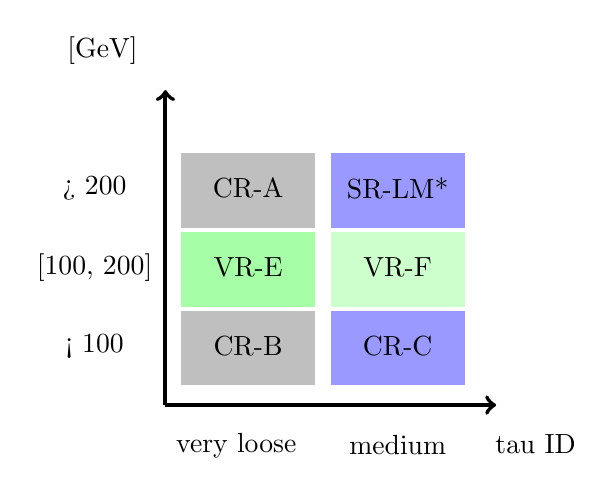
\begin{tikzpicture}
		\draw[line width =1.5pt,->] (0,0) -- (4.2,0);
		\node[](A) at (4.7,-0.5) {tau ID};
		\draw[line width =1.5pt,->] (0,0) -- (0,4.0);
		\node[](B) at (-0.8,4.5) {\Summt [GeV]};
		\node[](D) at (0.9, -0.51) {very loose };
		\node[](D) at (2.95, -0.50) {medium };
		\fill[gray!50] (0.2,0.25) rectangle (1.9,1.2);
		\node[](E) at (1.05,0.75) {CR-B};
		\node[](F)  at (-0.9,0.75) {< 100};
		\fill[green!35] (0.2,1.25) rectangle (1.9,2.2);
		\node[](G) at (1.05,1.75) {VR-E};
		\node[](H)  at (-0.9,1.75) {[100, 200]};
		\fill[gray!50] (0.2,2.25) rectangle (1.9,3.2);
		\node[](I) at (1.05,2.75) {CR-A};
		\node[](J)  at (-0.9,2.75) {> 200};
		\fill[blue!40] (2.1,0.25) rectangle (3.8,1.2);
		\node[](K) at (2.95,0.75) {CR-C};
		\fill[green!20] (2.1,1.25) rectangle (3.8,2.2);
		\node[](L) at (2.95,1.75) {VR-F};
		\fill[blue!40] (2.1,2.25) rectangle (3.8,3.2);
		\node[](M) at (2.95,2.75) {SR-LM*};
		\end{tikzpicture} }}
		  \subfloat[High mass ABCD regions]{
		\centering
	\scalebox{0.9}{
		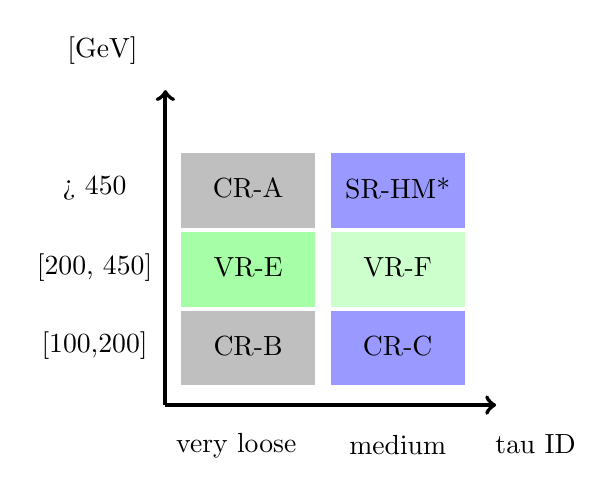
\begin{tikzpicture}
		\draw[line width =1.5pt,->] (0,0) -- (4.2,0);
		\node[](A) at (4.7,-0.5) {tau ID};
		\draw[line width =1.5pt,->] (0,0) -- (0,4.0);
		\node[](B) at (-0.8,4.5) {\Summt [GeV]};
		\node[](D) at (0.9, -0.51) {very loose };
		\node[](D) at (2.95, -0.50) {medium };
		\fill[gray!50] (0.2,0.25) rectangle (1.9,1.2);
		\node[](E) at (1.05,0.75) {CR-B};
		\node[](F)  at (-0.9,0.75) {[100,200]};
		\fill[green!35] (0.2,1.25) rectangle (1.9,2.2);
		\node[](G) at (1.05,1.75) {VR-E};
		\node[](H)  at (-0.9,1.75) {[200, 450]};
		\fill[gray!50] (0.2,2.25) rectangle (1.9,3.2);
		\node[](I) at (1.05,2.75) {CR-A};
		\node[](J)  at (-0.9,2.75) {> 450};
		\fill[blue!40] (2.1,0.25) rectangle (3.8,1.2);
		\node[](K) at (2.95,0.75) {CR-C};
		\fill[green!20] (2.1,1.25) rectangle (3.8,2.2);
		\node[](L) at (2.95,1.75) {VR-F};
		\fill[blue!40] (2.1,2.25) rectangle (3.8,3.2);
		\node[](M) at (2.95,2.75) {SR-HM*};
		\end{tikzpicture}}
}
\caption{ABCD region illustration for the low and high mass signal regions \label{fig:bkgestimation:QCD:sketch} Here only the cuts on \Summt and the tau-ID are shown.  $^*$ As described in section \ref{sec:analysis:sroptimisation},  further requirements on other kinematic variables are applied to define the signal regions}
\end{figure}

\begin{table}[ht!]
\centering
\footnotesize
\begin{tabular}{|c|c||c|c|}
\hline 
\textbf{CR-A} & \textbf{SR-LM} & \textbf{CR-A} & \textbf{SR-HM}\tabularnewline
\hline 
\hline 
$\geq$2 very loose or loose $\tau$'s & $\geq$2 medium $\tau$'s & $\geq$2 very loose or loose $\tau$'s & $\geq$2 medium $\tau$'s\tabularnewline
\textless{} 2 medium $\tau$'s & - & \textless{} 2 medium $\tau$'s & -\tabularnewline
$m_{Tsum}\geq200$ GeV & $m_{Tsum}\geq200$ GeV & $m_{Tsum}\geq450$ GeV & $m_{Tsum}\geq450$ GeV\tabularnewline
$\Delta\Phi(\tau_{1},\tau_{2})\geq1.5$ & $\Delta\Phi(\tau_{1},\tau_{2})\geq1.5$ & \Met $\geq$50 GeV & \Met $\geq$150 GeV\tabularnewline
\hline 
\hline 
\textbf{VR-E} & \textbf{VR-F} & \textbf{VR-E} & \textbf{VR-F}\tabularnewline
\hline 
\hline 
$\geq$2 very loose or loose $\tau$'s & $\geq$2 medium $\tau$'s & $\geq$2 very loose or loose $\tau$'s & $\geq$2 medium $\tau$'s\tabularnewline
\textless{} 2 medium $\tau$'s & - & \textless{} 2 medium $\tau$'s & -\tabularnewline
$m_{Tsum}$ $\in$ $[100,200]$ GeV & $m_{Tsum}$ $\in$ $[100,200]$ GeV & $m_{Tsum}$ $\in$ $[200,450]$ GeV & $m_{Tsum}$ $\in$ $[200,450]$ GeV\tabularnewline
$\Delta\Phi(\tau_{1},\tau_{2})\leq1.5$ & $\Delta\Phi(\tau_{1},\tau_{2})\leq1.5$ & \Met $\geq$50 GeV & \Met $\geq$50 GeV\tabularnewline
\hline 
\hline 
\textbf{CR-B} & \textbf{CR-C} & \textbf{CR-B} & \textbf{CR-C}\tabularnewline
\hline 
\hline 
$\geq$2 very loose or loose $\tau$'s & $\geq$2 medium $\tau$'s & $\geq$2 very loose or loose $\tau$'s & $\geq$2 medium $\tau$'s\tabularnewline
\textless{} 2 medium $\tau$'s & - & \textless{} 2 medium $\tau$'s & -\tabularnewline
$m_{Tsum}<100$ GeV & $m_{Tsum}<100$ GeV & $m_{Tsum}$ $\in$ $[100,200]$ GeV & $m_{Tsum}$ $\in$ $[100,200]$ GeV\tabularnewline
$\Delta\Phi(\tau_{1},\tau_{2})\leq1.5$ & $\Delta\Phi(\tau_{1},\tau_{2})\leq1.5$ & \Met $\geq$50 GeV & \Met $\geq$50 GeV\tabularnewline
\hline 
\end{tabular}
\caption{The multi-jet control region and validation region
  definitions for signal regions described in Table~\ref{tab:SRdef}.
  Only those requirements regarding the \Summt that are different in the CRs/VRs with
  respect to the SRs are listed. \label{tab:bkgestimation:QCD:table}}
\end{table}

%
%\begin{table}[ht!]
%\centering
%\footnotesize
%\smallskip
%\begin{tabular}{c|c}
%\toprule
%% AD------------------
%$\mathbf {CR-A~}$ & $\mathbf {SR-LM}$\\
%\hline
%$\ge$ 2 very loose or loose $\tau$s       & $\ge$ 2 medium $\tau$s (SS)   \\
%$<$ 2 medium $\tau$s     &      --      \\
%$m_{Tsum}\geq 200 \text{ GeV} $ &  $m_{Tsum}\geq 200 \text{ GeV} $      \\ %SumMtCut
%$\Delta \Phi(\tau_1,\tau_2) \geq 1.5 $ &  $\Delta \Phi(\tau_1,\tau_2) \geq 1.5 $ \\ %DeltaPhiCut
%\hline
%%EF---------------
%\hline
%$\mathbf {VR-E~}$ & $\mathbf {VR-F~}$ \\
%\hline                                                      \hline
%$\ge$ 2 very loose or loose $\tau$s       & $\ge$ 2 medium $\tau$s (SS)   \\
%$<$ 2 medium $\tau$s     &      --      \\
%$m_{Tsum}\in [100,200] \text{ GeV} $ &  $m_{Tsum}\in [100,200] \text{ GeV} $      \\ %SumMtCut
%$\Delta \Phi(\tau_1,\tau_2) \leq 1.5 $ &  $\Delta \Phi(\tau_1,\tau_2) \leq 1.5 $ \\ %DeltaPhiCut
%\hline
%% BC-----------------
%\hline
%$\mathbf {CR-B~}$ & $\mathbf {CR-C~}$ \\
%\hline                                                      \hline
%$\ge$ 2 very loose or loose $\tau$s       &  $\ge$ 2 medium $\tau$s (SS)   \\
%$<$ 2 medium $\tau$s     &      --      \\
%$m_{Tsum}< 100 \text{ GeV} $ &  $m_{Tsum}< 100 \text{ GeV} $      \\ %SumMtCut
%$\Delta \Phi(\tau_1,\tau_2) \leq 1.5 $ &  $\Delta \Phi(\tau_1,\tau_2) \leq 1.5 $ \\ %DeltaPhiCut
%\hline
%\bottomrule
%\end{tabular}
%\smallskip
%\begin{tabular}{c|c}
%\toprule
%% AD------------------
%$\mathbf {CR-A~}$ & $\mathbf {SR-HM}$\\
%\hline
%$\ge$ 2 very loose or loose $\tau$s       & $\ge$ 2 medium $\tau$s (SS)   \\
%$<$ 2 medium $\tau$s     &      --      \\
%$m_{Tsum}\geq 450 \text{ GeV} $ &  $m_{Tsum}\geq 450 \text{ GeV} $      \\ %SumMtCut
%$E_T^\text{miss} \geq 50 \text{ GeV} $ & $E_T^\text{miss} \geq 150 \text{ GeV} $ \\ %met cut
%\hline
%%EF---------------
%\hline
%$\mathbf {VR-E~}$ & $\mathbf {VR-F~}$\\
%\hline                                                      \hline
%$\ge$ 2 very loose or loose $\tau$s       & $\ge$ 2 medium $\tau$s (SS)   \\
%$<$ 2 medium $\tau$s     &      --      \\
%$m_{Tsum}\in [200,450] \text{ GeV} $ &  $m_{Tsum}\in [200,450] \text{ GeV} $      \\ %SumMtCut
%$E_T^\text{miss} \geq 50 \text{ GeV} $ & $E_T^\text{miss} \geq 50 \text{ GeV} $ \\ %met cut
%\hline
%% BC-----------------
%\hline
%$\mathbf {CR-B~}$ & $\mathbf {CR-C~}$ \\
%\hline                                                      \hline
%$\ge$ 2 very loose or loose $\tau$s       &  $\ge$ 2 medium $\tau$s (SS)   \\
%$<$ 2 medium $\tau$s     &      --      \\
%$m_{Tsum} \in [100,200] \text{ GeV} $ &  $m_{Tsum} \in [100,200] \text{ GeV} $      \\ %SumMtCut
%$E_T^\text{miss} \geq 50 \text{ GeV} $ & $E_T^\text{miss} \geq 50 \text{ GeV} $ \\ %met cut
%\hline
%\bottomrule
%\end{tabular}
%\caption{The multi-jet control region and validation region
%  definitions for signal regions described in Table~\ref{tab:SRdef}.
%  Only those requirements regarding the \Summt that are different in the CRs/VRs with
%  respect to the SRs are listed. \label{tab:bkgestimation:QCD:table}}
%\end{table}

The multi-jet (MJ) contribution in CR-B and CR-C is obtained from the data yields in the respective regions,  with all other background contributions from Monte Carlo simulation subtracted;

\begin{align}
N^{MJ}_{CR-B/C} =  N^{data}_{CR-B/C} - N^{MC}_{CR-B/C} 
\end{align}

a transfer factor is extracted from the yields in CR-B and CR-C to extrapolate the multi-jet contribution to the medium ID validation and signal regions (VR-F and SR). 

\begin{align}
TF = \frac{N^{MJ}_{CR-C}}{N^{MJ}_{CR-B}}
\label{eq:bkgestimation:TF}
\end{align}

The systematic uncertainty on the transfer factor is estimated in the validation regions using formula \eqref{eq:bkgestimation:deltaTF} and is visualised in Figure \ref{fig:bkgestimation:ABCD:TF}.

\begin{align}
\Delta(TF)_{sys} =  | \frac{N^{MJ}_{CR-C}}{N^{MJ}_{CR-B}} - \frac{N^{MJ}_{VR-F}}{N^{MJ}_{VR-E}} | \label{eq:bkgestimation:deltaTF}
\end{align}

\begin{figure}[!htpb]
  \centering
%\subfloat[Low Mass]{\includegraphics[width=0.45\textwidth]{figures/C1N2SS/ABCD_closures/TF_SumMt_asymMT2False.pdf}}
\subfloat[Low Mass]{\includegraphics[width=0.45\textwidth]{figures/C1N2SS/ABCD_closures_noATLAS/TF_SumMtADT_asymMT2False.pdf}}
%\subfloat[High Mass]{\includegraphics[width=0.45\textwidth]{figures/C1N2SS/ABCD_closures/TF_SumMt_ditauMETMT2False.pdf}}
\subfloat[High Mass]{\includegraphics[width=0.45\textwidth]{figures/C1N2SS/ABCD_closures_noATLAS/TF_SumMtDTM_ditauMETMT2False.pdf}}
\caption{Dependency of the transfer factor on \Summt for low mass and high mass regions. Highlighted in the lower panel in red is the nominal used transfer factor value. All uncertainties are statistical only. \label{fig:bkgestimation:ABCD:TF}}
\end{figure}

%%----- result
The multi-jet yield in the signal region is then given by the multi-jet contribution in CR-A (given through data subtracted by other \ac{SM} contributions from Monte Carlo simulation) multiplied by the transfer factor with additional cuts.
The results of the ABCD method are summarised in Table
\ref{tab:bkgestimation:ABCDresults}. The SM predictions are in agreement with
the observed data counts in the multi-jet validation regions, as shown in Table \ref{tab:bkgestimation:VRFresults}.
%The systematic uncertainties of the ABCD method are discussed in
%Section \ref{sec:syst_ABCD}.

%\begin{table}
%\centering
%\tiny
%  \begin{tabular}{c|c|c|c|c|c|c|c|c}
%  \hline
%  & Sample & CR-B & CR-C & VR-E & CR-A & T=C/B & multi-jet in VR-F & multi-jet in SR-D\tabularnewline
%  \hline
%  \hline
%  \multirow{7}{*}{LM} & \textbf{Data} & \textbf{585} & \textbf{65} & \textbf{356} & \textbf{1505} & \multirow{2}{*}{} & \multirow{7}{*}{$19.55 \pm 1.13$} & \multirow{7}{*}{$0.94\pm0.27$}\tabularnewline
%%  \cline{2-2}
%   & $Z$+ jets & $11.70\pm2.11$ & $25.92\pm2.70$ & $3.62\pm1.06$ & $32.85\pm11.07$ &  &  & \tabularnewline
%  \cline{2-2}
%   & $W$+ jets & $4.84\pm2.35$ & $3.29\pm0.96$ & $11.48\pm4.67$ & $32.21\pm10.06$ & $0.058$ &  & \tabularnewline
%  \cline{2-2}
%   & Multiboson & $0.80\pm0.38$ & $2.04\pm0.35$ & $1.20\pm0.40$ & $2.18\pm0.50$ & $\pm0.015$ &  & \tabularnewline
%  \cline{2-2}
%   & Top & $2.54\pm0.75$ & $0.16\pm0.27$ & $2.45\pm0.88$ & $5.24\pm0.93$ & $\pm0.020$ &  & \tabularnewline
%  \cline{2-2}
%   & Higgs & $0.13\pm0.04$ & $0.73\pm0.09$ & $0.09\pm0.05$ & $0.53\pm0.46$ & \multirow{2}{*}{} &  & \tabularnewline
%  \cline{2-2}
%   & \emph{Multi-jet} & $564.98\pm24.41$ & $32.86\pm8.57$ & $337.16\pm19.49$ & $1431.98\pm41.59$ &  &  & \tabularnewline
%  \hline
%  \hline
%  \multirow{7}{*}{HM} & \textbf{Data} & \textbf{2185} & \textbf{309} & \textbf{3651} & \textbf{14} & \multirow{2}{*}{} & \multirow{7}{*}{$283.10 \pm 7.738$} & \multirow{7}{*}{$-0.086\pm0.31$}\tabularnewline
%  \cline{2-2}
%   & $Z$+ jets & $30.81\pm7.41$ & $32.53\pm10.81$ & $56.12\pm17.74$ & $2.64\pm1.37$ &  &  & \tabularnewline
%  \cline{2-2}
%   & $W$+ jets & $178.87\pm51.40$ & $74.13\pm15.33$ & $248.68\pm64.10$ & $6.35\pm2.58$ & $0.086$ &  & \tabularnewline
%  \cline{2-2}
%   & Multiboson & $6.03\pm0.87$ & $18.35\pm0.97$ & $14.42\pm1.44$ & $0.83\pm0.29$ & $\pm0.014$ &  & \tabularnewline
%  \cline{2-2}
%   & Top & $20.73\pm2.01$ & $14.38\pm1.53$ & $39.23\pm2.72$ & $2.10\pm0.57$ & $\pm0.011$ &  & \tabularnewline
%  \cline{2-2}
%   & Higgs & $0.53\pm0.38$ & $1.27\pm0.58$ & $0.71\pm0.47$ & $0.01\pm0.00$ & \multirow{2}{*}{} &  & \tabularnewline
%  \cline{2-2}
%   & \emph{Multi-jet} & $1948.04\pm69.90$ & $168.34\pm25.78$ & $3291.83\pm89.91$ & $2.07\pm4.79$ &  &  & \tabularnewline
%  \hline
%  \end{tabular}
%  \caption{Monte Carlo  backgrounds in the ABCD regions of the signal
%  regions defined in Table \ref{tab:SRdef}. The uncertainties given
%  on the transfer factor are both statistical and systematic
%  uncertainties. \label{tab:bkgestimation:ABCDresults} }
%\end{table}

\begin{table}
\centering {\tiny{}}%
\begin{tabular}{|c|c|c|c|c|c|c|c|c|}
\hline 
\multirow{2}{*}{} & \multirow{2}{*}{\textbf{\tiny{}Sample }} & \multirow{2}{*}{\textbf{\tiny{}CR-B }} & \multirow{2}{*}{\textbf{\tiny{}CR-C }} & \multirow{2}{*}{\textbf{\tiny{}VR-E }} & \multirow{2}{*}{\textbf{\tiny{}CR-A }} & \multirow{2}{*}{\textbf{\tiny{}T=C/B}{\tiny{} }} & \textbf{\tiny{}multi-jet } & \textbf{\tiny{}multi-jet }\tabularnewline
 &  &  &  &  &  &  & \textbf{\tiny{}in VR-F } & \textbf{\tiny{}in SR-C1N2SS}\tabularnewline
\hline 
\hline 
\multirow{7}{*}{\textbf{\tiny{}LM}} & \textbf{\tiny{}Data}{\tiny{} } & \textbf{\tiny{}585}{\tiny{} } & \textbf{\tiny{}65}{\tiny{} } & \textbf{\tiny{}356}{\tiny{} } & \textbf{\tiny{}1505}{\tiny{} } & \multirow{2}{*}{} & \multirow{7}{*}{{\tiny{}$19.55\pm1.13$}} & \multirow{7}{*}{{\tiny{}$0.94\pm0.27$}}\tabularnewline
\cline{2-6} \cline{3-6} \cline{4-6} \cline{5-6} \cline{6-6} 
 & {\tiny{}$Z$+ jets } & {\tiny{}$11.70\pm2.11$ } & {\tiny{}$25.92\pm2.70$ } & {\tiny{}$3.62\pm1.06$ } & {\tiny{}$32.85\pm11.07$ } &  &  & \tabularnewline
\cline{2-6} \cline{3-6} \cline{4-6} \cline{5-6} \cline{6-6} 
 & {\tiny{}$W$+ jets } & {\tiny{}$4.84\pm2.35$ } & {\tiny{}$3.29\pm0.96$ } & {\tiny{}$11.48\pm4.67$ } & {\tiny{}$32.21\pm10.06$ } & {\tiny{}$0.058$ } &  & \tabularnewline
\cline{2-6} \cline{3-6} \cline{4-6} \cline{5-6} \cline{6-6} 
 & {\tiny{}Multi-boson } & {\tiny{}$0.80\pm0.38$ } & {\tiny{}$2.04\pm0.35$ } & {\tiny{}$1.20\pm0.40$ } & {\tiny{}$2.18\pm0.50$ } & {\tiny{}$\pm0.015$ } &  & \tabularnewline
\cline{2-6} \cline{3-6} \cline{4-6} \cline{5-6} \cline{6-6} 
 & {\tiny{}Top } & {\tiny{}$2.54\pm0.75$ } & {\tiny{}$0.16\pm0.27$ } & {\tiny{}$2.45\pm0.88$ } & {\tiny{}$5.24\pm0.93$ } & {\tiny{}$\pm0.020$ } &  & \tabularnewline
\cline{2-6} \cline{3-6} \cline{4-6} \cline{5-6} \cline{6-6} 
 & {\tiny{}Higgs } & {\tiny{}$0.13\pm0.04$ } & {\tiny{}$0.73\pm0.09$ } & {\tiny{}$0.09\pm0.05$ } & {\tiny{}$0.53\pm0.46$ } & \multirow{2}{*}{} &  & \tabularnewline
\cline{2-6} \cline{3-6} \cline{4-6} \cline{5-6} \cline{6-6} 
 & \emph{\tiny{}Multi-jet}{\tiny{} } & {\tiny{}$564.98\pm24.41$ } & {\tiny{}$32.86\pm8.57$ } & {\tiny{}$337.16\pm19.49$ } & {\tiny{}$1431.98\pm41.59$ } &  &  & \tabularnewline
\hline 
\multirow{7}{*}{\textbf{\tiny{}HM}} & \textbf{\tiny{}Data}{\tiny{} } & \textbf{\tiny{}2185}{\tiny{} } & \textbf{\tiny{}309}{\tiny{} } & \textbf{\tiny{}3651}{\tiny{} } & \textbf{\tiny{}14}{\tiny{} } & \multirow{2}{*}{} & \multirow{7}{*}{{\tiny{}$283.10\pm7.738$}} & \multirow{7}{*}{{\tiny{}$-0.086\pm0.31$}}\tabularnewline
\cline{2-6} \cline{3-6} \cline{4-6} \cline{5-6} \cline{6-6} 
 & {\tiny{}$Z$+ jets } & {\tiny{}$30.81\pm7.41$ } & {\tiny{}$32.53\pm10.81$ } & {\tiny{}$56.12\pm17.74$ } & {\tiny{}$2.64\pm1.37$ } &  &  & \tabularnewline
\cline{2-6} \cline{3-6} \cline{4-6} \cline{5-6} \cline{6-6} 
 & {\tiny{}$W$+ jets } & {\tiny{}$178.87\pm51.40$ } & {\tiny{}$74.13\pm15.33$ } & {\tiny{}$248.68\pm64.10$ } & {\tiny{}$6.35\pm2.58$ } & {\tiny{}$0.086$ } &  & \tabularnewline
\cline{2-6} \cline{3-6} \cline{4-6} \cline{5-6} \cline{6-6} 
 & {\tiny{}Multi-boson } & {\tiny{}$6.03\pm0.87$ } & {\tiny{}$18.35\pm0.97$ } & {\tiny{}$14.42\pm1.44$ } & {\tiny{}$0.83\pm0.29$ } & {\tiny{}$\pm0.014$ } &  & \tabularnewline
\cline{2-6} \cline{3-6} \cline{4-6} \cline{5-6} \cline{6-6} 
 & {\tiny{}Top } & {\tiny{}$20.73\pm2.01$ } & {\tiny{}$14.38\pm1.53$ } & {\tiny{}$39.23\pm2.72$ } & {\tiny{}$2.10\pm0.57$ } & {\tiny{}$\pm0.011$ } &  & \tabularnewline
\cline{2-6} \cline{3-6} \cline{4-6} \cline{5-6} \cline{6-6} 
 & {\tiny{}Higgs } & {\tiny{}$0.53\pm0.38$ } & {\tiny{}$1.27\pm0.58$ } & {\tiny{}$0.71\pm0.47$ } & {\tiny{}$0.01\pm0.00$ } & \multirow{2}{*}{} &  & \tabularnewline
\cline{2-6} \cline{3-6} \cline{4-6} \cline{5-6} \cline{6-6} 
 & \emph{\tiny{}Multi-jet}{\tiny{} } & {\tiny{}$1948.04\pm69.90$ } & {\tiny{}$168.34\pm25.78$ } & {\tiny{}$3291.83\pm89.91$ } & {\tiny{}$2.07\pm4.79$ } &  &  & \tabularnewline
\hline 
\end{tabular}{\tiny{}\caption{Monte Carlo backgrounds in the ABCD regions of the signal regions
defined in Table \ref{tab:SRdef}. The uncertainties given on the
transfer factor are  statistical followed by systematic uncertainties.
\label{tab:bkgestimation:ABCDresults} }
}
\end{table}


\begin{table}
\centering
\begin{tabular}{|c|c|c|}
\hline
Sample & VRF-LM& VRF-HM\\
\hline
\hline
W+jets & $1.35\pm0.88$ & $149.75\pm42.98$\\
\hline
Z+jets & $9.30\pm1.30$ & $36.82\pm19.62$\\
\hline
top & $0.99\pm0.48$ & $19.78\pm1.85$\\
\hline
Muliboson & $1.47\pm0.35$ & $26.31\pm1.2$\\
\hline
Higgs & $0.25\pm0.06$ & $3.16\pm1.13$\\
\hline
multi-jet & $19.55 \pm 1.13$ & $283.10 \pm 7.73$\\
\hline
\hline
SM total & $32.92 \pm 2.02$ & $518.92 \pm 47.94$\\
\hline
\textbf{Data} & \textbf{40} & \textbf{484}\\
\hline
\end{tabular}
\caption{Event yields in VR-F-LM and VR-F-HM. Only statistical
  uncertainties are included in the multi-jet 
  yield.  \label{tab:bkgestimation:VRFresults}%\textcolor{red}{Check ABCD validation, large disagreement}
}
\end{table}

%\textcolor{red}{distribution for Direct Stau validations to be added!}
In Figure \ref{fig:QCD-VR-LowMass-ss} (Figure \ref{fig:QCD-VR-highMass-ss}) ,
distributions of the relevant kinematic variables are shown for data,
SM expectations and illustrative SUSY benchmark models for the
multi-jet validation regions VR-F-LM (VR-F-HM).  The multi-jet contribution in VR-F is given through the multijet contribution in VR-E (as data subtracted by other \ac{SM} contributions) times the transfer factor as defined in equation \eqref{eq:bkgestimation:TF}. The signal contamination in VR-F-LM is below 10\%,  in VR-F-HM below 30\%. The SM background distributions are taken from MC
simulation, except for the multi-jet contribution, which is estimated using the ABCD method
described above. 
The distributions include statistical and systematic error on the ABCD method added in quadrature.
Reasonable data and SM agreement are observed within uncertainty and show good extrapolation in \Mttwomax.

%--------------------------------------------------------------------
\begin{figure}[!htpb]
\centering
  \subfloat[]{\includegraphics[width=0.45\textwidth]{figures/UpdatedThesisFigures/VRFLM_Prefit_noATLAS/asymVRF_wDPhiOnly_noLLV_mt2maxvrfL.pdf}}
  \subfloat[]{\includegraphics[width=0.45\textwidth]{figures/UpdatedThesisFigures/VRFLM_Prefit_noATLAS/VRFLM_met.pdf}}\\
 \subfloat[]{\includegraphics[width=0.45\textwidth]{figures/UpdatedThesisFigures/VRFLM_Prefit_noATLAS/asymVRF_wDPhiOnly_noLLV_SumMtTauVRFLM.pdf}}
   \subfloat[]{\includegraphics[width=0.45\textwidth]{figures/UpdatedThesisFigures/VRFLM_Prefit_noATLAS/asymVRF_wDPhiOnly_noLLV_mvisTauTauSRH_improved.pdf}}\\
%  \subfloat[]{\includegraphics[width=0.45\textwidth]{figures/C1N2SS/ABCD_low/asymVRF_wDPhiOnly_noLLV_signaljets.pdf}}
 % \subfloat[]{\includegraphics[width=0.45\textwidth]{figures/C1N2SS/ABCD_low/asymVRF_wDPhiOnly_noLLV_deltaPhiTau1Met.pdf}}\\
  \subfloat[]{\includegraphics[width=0.45\textwidth]{figures/UpdatedThesisFigures/VRFLM_Prefit_noATLAS/asymVRF_wDPhiOnly_noLLV_tau1PtVRFLtrigLim_improved.pdf}}
  \subfloat[]{\includegraphics[width=0.45\textwidth]{figures/UpdatedThesisFigures/VRFLM_Prefit_noATLAS/asymVRF_wDPhiOnly_noLLV_tau2PtSRH_improved.pdf}}
  %\subfloat[]{\includegraphics[width=0.45\textwidth]{figures/C1N2SS/ABCD_low/asymVRF_wDPhiOnly_noLLV_nbjets.pdf}}
  \caption{Data/MC distributions in VR-F-LM, the uncertainty band includes statistical and systematic uncertainties. 
\label{fig:QCD-VR-LowMass-ss}}
\end{figure} %\addtocounter{figure}{-1}

\begin{figure}[!htpb]
\centering
  \subfloat[]{\includegraphics[width=0.45\textwidth]{figures/UpdatedThesisFigures/VRFHM_Prefit_noATLAS/ditauMETVRFSumMtlowMet_plateau_mt2maxvrfH_improved.pdf}}
  \subfloat[]{\includegraphics[width=0.45\textwidth]{figures/UpdatedThesisFigures/VRFHM_Prefit_noATLAS/ditauMETVRFSumMtlowMet_plateau_metVRFH.pdf}}\\
   \subfloat[]{\includegraphics[width=0.45\textwidth]{figures/UpdatedThesisFigures/VRFHM_Prefit_noATLAS/ditauMETVRFSumMtlowMet_plateau_SumMtTauVRFHM_5b.pdf}}
  \subfloat[]{\includegraphics[width=0.45\textwidth]{figures/UpdatedThesisFigures/VRFHM_Prefit_noATLAS/ditauMETVRFSumMtlowMet_plateau_mvisTauTau100.pdf}}\\
  %\subfloat[]{\includegraphics[width=0.45\textwidth]{figures/C1N2SS/ABCD_high/ditauMETVRFSumMtlowMet_plateau_signaljets.pdf}}
  %\subfloat[]{\includegraphics[width=0.45\textwidth]{figures/C1N2SS/ABCD_high/ditauMETVRFSumMtlowMet_plateau_deltaPhiTau1Met.pdf}}\\
  \subfloat[]{\includegraphics[width=0.45\textwidth]{figures/UpdatedThesisFigures/VRFHM_Prefit_noATLAS/ditauMETVRFSumMtlowMet_plateau_tau1PtVRFH_improved.pdf}}
  \subfloat[]{\includegraphics[width=0.45\textwidth]{figures/UpdatedThesisFigures/VRFHM_Prefit_noATLAS/ditauMETVRFSumMtlowMet_plateau_tau2PtSRH_improved.pdf}}
 % \subfloat[]{\includegraphics[width=0.45\textwidth]{figures/C1N2SS/ABCD_high/ditauMETVRFSumMtlowMet_plateau_nbjets.pdf}}
  \caption{Data/MC distributions in VR-F-HM, the uncertainty band includes statistical and systematic uncertainties. 
\label{fig:QCD-VR-highMass-ss}}
\end{figure}

\pagebreak
\clearpage
\subsection{Estimation of W+jets background}
\label{sec:SS:Wjets}
%====================================================================================================
%==============================================W+jets estimation ==================================
%====================================================================================================
\FloatBarrier
The production of a W boson in association with a jet can enter a di-tau final state if one or more of the associated jets is misidentified as hadronic decaying tau lepton.  The W+jets background contributes to both low and high mass signal regions,  through moderate \Met contributions of the neutrinos in the W bosons decay and mismeasured \Met. 
A control and validation region targetting both signal regions is defined to estimate this background.  A summary of the requirements applied to define the regions is given in Table \ref{tab:bkgestimation:WCRVR}.
A final state with precisely one hadronically decaying tau lepton and one muon,  both with the same electric charge,  is selected to increase the available statistics. 
This final state targets to model events entering the signal regions with at least one fake tau,  replacing the prompt tau through a prompt muon. 
A veto on baseline electrons is applied to target the muon plus hadronic tau final state.
A veto on b-jets is used to constrain contributions from top related processes,  whereas a cut on the transverse mass of the muon is used to remove Z+jets contaminations. 
A lower cut on the \Met of 50 GeV is used to veto events with very close by muons and taus,  which accumulate at low \Met due to failed separation in overlap removal procedures.  A cut on the \Mttwo variable,  built with the muon and tau,  is required to achieve similar event structures and phase spaces to the signal regions. 
This mimics the kinematic restrictions on the two leading taus used in the signal regions.

\begin{table}[!htpb]
\centering
\begin{tabular}{|c|c|} \hline
$W$-CR                 & $W$-VR \\ \hline
\multicolumn{2}{|c|}{pass TrigHLT\_mu20\_iloose\_L1MU15 (2015) and HLT\_mu26\_ivarmedium (2016-2018)} \\
\multicolumn{2}{|c|}{$==$ 1 medium tau and 1 isolated muon (SS) } \\
\multicolumn{2}{|c|}{baseline electron veto}\\
\multicolumn{2}{|c|}{$b$-veto}\\
\multicolumn{2}{|c|}{$50 < \text{m}_{\text{T}}(\mu)<150\,\text{GeV}$}\\
\multicolumn{2}{|c|}{$\text{m}_{\text{T}}(\tau)+\text{m}_{\text{T}}(\mu)>80\,\text{GeV}$}\\
%\multicolumn{2}{|c|}{$ m_T(\mu) \in [50, 150]$}\\
%\multicolumn{2}{|c|}{$ m_T(\mu) + m_T(\tau_1) \geq 80 \text{ GeV}$}\\
\multicolumn{2}{|c|}{$E_T^\text{miss} > 50 \text{ GeV}$}\\
$m_{T2}(\mu,\tau) <  60 \text{ GeV}$ & $m_{T2}(\mu, \tau) \geq 60 \text{ GeV}$\\ \hline
\end{tabular}\caption{Wjets control and validation region definition \label{tab:bkgestimation:WCRVR}}
\end{table}

With the cuts specified in Table \ref{tab:bkgestimation:WCRVR},  control and validation regions with high statistics are constructed, with a breakdown of the background yields, estimated purely from Monte Carlo simulation, which can be seen in table \ref{tab:bkgestimation:WCRVRyields}.
The yield does not include systematic uncertainties.  Both control and validation region show a high purity in W+jets processes,  above 80$\%$ in both cases,  as shown in figure \ref{fig:bkgestimation:WCRVRpurity}.  The signal contamination in both regions is negligible(see Fig.  \ref{fig:SS:WCRVRcontamination}). Kinematic distributions in the W-CR and W-VR are shown in Figure \ref{fig:SS:WCR} and \ref{fig:bkgestimation:wvrmcdata}, respectively. 

\begin{table}
  \centering
\begin{tabular}{|c|c|c|}
\hline
Sample & W-CR & W-VR\tabularnewline
\hline
\hline
W+jets & $ 21005.90 \pm 880.74 $ & $ 5852.23 \pm 502.55 $\tabularnewline
\hline
Z+jets  & $ 2529.68 \pm 205.40 $& $ 737.16 \pm 90.34 $\tabularnewline
\hline
top & $ 1148.86 \pm 12.66 $ & $ 185.39 \pm 5.18 $\tabularnewline
\hline
Multiboson & $ 629.41 \pm 8.79 $ & $ 122.50 \pm 3.62 $\tabularnewline
\hline
Higgs & $ 20.70 \pm 3.31 $ & $ 5.49 \pm 1.72 $\tabularnewline
\hline
Multi-jet & $0.00\pm0.00$ & $0.00\pm0.00$\tabularnewline
\hline
\hline
SM total & $ 25334.55 \pm 904.51 $ & $ 6902.76 \pm 510.65 $\tabularnewline
\hline
\textbf{Data} & \textbf{$\mathbf{25728}$} & $\mathbf{6662}$\tabularnewline
\hline
\end{tabular}
\caption{Event yields in W+jets Control and Validation region. The shown uncertainties for SM backgrounds are the statistical
uncertainties only.  \label{tab:bkgestimation:WCRVRyields}}
\end{table}

\begin{figure}[!htpb]
\centering
  \includegraphics[width=0.95\textwidth]{figures/UpdatedThesisFigures/WCRVR_piechart.png}
  \caption{Background composition in W+jet Control and Validation region \label{fig:bkgestimation:WCRVRpurity}}\end{figure}


\begin{figure}[!htpb]
  \centering
  \subfloat[W-CR]{\includegraphics[width=0.49\textwidth]{figures/C1N2SS/WVRCR_muWeight/SigBkgTrue_QCDtrFalse_MjFalseWCR_public_wolowMt2_vetobaselineelec_met.Syst_bkup_nonumbers.pdf}}
  \subfloat[W-VR]{\includegraphics[width=0.49\textwidth]{figures/C1N2SS/WVRCR_muWeight/SigBkgTrue_QCDtrFalse_MjFalseWVR_public_vetobaselineelec_met.Syst_bkup_nonumbers.pdf}}
\caption{Signal contamination in percentage in W-CR and W-VR. \label{fig:SS:WCRVRcontamination}}
\end{figure}

\begin{figure}[!htpb]
\centering
  \subfloat[]{\includegraphics[width=0.45\textwidth]{figures/UpdatedThesisFigures_noATLAS/WCR_Prefit/singlemuWCR_public_wolowMt2_vetobaselineelec_met_emtmt2max_wcr.pdf}}
  \subfloat[]{\includegraphics[width=0.45\textwidth]{figures/UpdatedThesisFigures_noATLAS/WCR_Prefit/singlemuWCR_public_wolowMt2_vetobaselineelec_met_metVRFH.pdf}}\\
  \subfloat[]{\includegraphics[width=0.45\textwidth]{figures/UpdatedThesisFigures_noATLAS/WCR_Prefit/singlemuWCR_public_wolowMt2_vetobaselineelec_met_muon_MTwcrvr.pdf}}
 % \subfloat[]{\includegraphics[width=0.45\textwidth]{figures/C1N2SS/WVRCR/singlemuWCR_public_wolowMt2_vetobaselineelec_met_signaljets.pdf}}
  \subfloat[]{\includegraphics[width=0.45\textwidth]{figures/UpdatedThesisFigures_noATLAS/WCR_Prefit/singlemuWCR_public_wolowMt2_vetobaselineelec_met_SumMtTauMuwcrvrshorter_improved.pdf}}\\
  %\subfloat[]{\includegraphics[width=0.45\textwidth]{figures/C1N2SS/WVRCR/singlemuWCR_public_wolowMt2_vetobaselineelec_met_deltaPhiTau1Met.pdf}}\\
  \subfloat[]{\includegraphics[width=0.45\textwidth]{figures/UpdatedThesisFigures_noATLAS/WCR_Prefit/singlemuWCR_public_wolowMt2_vetobaselineelec_met_tau1PtVRFH_improved.pdf}}
  \subfloat[]{\includegraphics[width=0.45\textwidth]{figures/UpdatedThesisFigures_noATLAS/WCR_Prefit/singlemuWCR_public_wolowMt2_vetobaselineelec_met_mu1Ptwcrvr_improved.pdf}}
  %\subfloat[]{\includegraphics[width=0.45\textwidth]{figures/C1N2SS/WVRCR/singlemuWCR_public_wolowMt2_nbjets.pdf}}
 \caption{ Distributions of  relevant kinematic variables in the $W$-CR.
The SM backgrounds other than multi-jet production are estimated from MC simulation
and normalised to 139~\ifb.
The hatched bands represent the statistical uncertainties and systematic uncertainties discussed in \ref{sec:analysis:systematics}.
%  The hatched bands represent the combined statistical and systematic uncertainties on the total SM background.
%For illustration, the distributions of the SUSY reference points are also shown as dashed lines.
The lower panel shows the ratio of data to the SM background estimate. \label{fig:SS:WCR} 
}
% \caption{W+jets control region data/MC distributions \label{fig:SS:WCR}}
\end{figure}

\begin{figure}[!htpb]
\centering
  \subfloat[]{\includegraphics[width=0.49\textwidth]{figures/UpdatedThesisFigures/WVR_Prefit_noATLAS/singlemuWVR_public_vetobaselineelec_met_emtmt2max_wvr_improved.pdf}}
  \subfloat[]{\includegraphics[width=0.49\textwidth]{figures/UpdatedThesisFigures/WVR_Prefit_noATLAS/singlemuWVR_public_vetobaselineelec_met_metWCRVR.pdf}}\\
  \subfloat[]{\includegraphics[width=0.49\textwidth]{figures/UpdatedThesisFigures/WVR_Prefit_noATLAS/WVR_muonmt.pdf}}
  %\subfloat[]{\includegraphics[width=0.49\textwidth]{figures/C1N2SS/WVRCR/singlemuWVR_public_vetobaselineelec_met_signaljets.pdf}}
  \subfloat[]{\includegraphics[width=0.49\textwidth]{figures/UpdatedThesisFigures/WVR_Prefit_noATLAS/singlemuWVR_public_vetobaselineelec_met_SumMtTauMuwcrvrshorter_improved.pdf}}\\
  %\subfloat[]{\includegraphics[width=0.49\textwidth]{figures/C1N2SS/WVRCR/singlemuWVR_public_vetobaselineelec_met_deltaPhiTau1Met.pdf}}\\
  \subfloat[]{\includegraphics[width=0.49\textwidth]{figures/UpdatedThesisFigures/WVR_Prefit_noATLAS/singlemuWVR_public_vetobaselineelec_met_tau1PtVRFH_improved.pdf}}
  \subfloat[]{\includegraphics[width=0.49\textwidth]{figures/UpdatedThesisFigures/WVR_Prefit_noATLAS/singlemuWVR_public_vetobaselineelec_met_mu1Ptwcrvr_improved.pdf}}
  %\subfloat[]{\includegraphics[width=0.49\textwidth]{figures/C1N2SS/WVRCR/singlemuWVR_public_nbjets.pdf}}
  %\caption{W+jets control region data/MC distributions \label{fig:SS:WVR}}
\caption{ Distributions of  relevant kinematic variables in the $W$-VR. The SM backgrounds other than multi-jet production are estimated from MC simulation and normalised to 139~\ifb.
The hatched bands represent the statistical uncertainties and systematic uncertainties discussed in \ref{sec:analysis:systematics}.
%   The hatched bands represent the combined statistical and systematic uncertainties on the total SM background.
%For illustration, the distributions of the SUSY reference points are also shown as dashed lines.
The lower panel shows the ratio of data to the SM background estimate. \label{fig:bkgestimation:wvrmcdata} 
}
\end{figure}

\pagebreak
\clearpage

%================================================================================================
%==============================================Top estimation =======================================
%=================================================================================================
\subsection{Top background estimation}
\label{sec:SS:Top}
\FloatBarrier
Top-related processes are a dominant background contribution, especially in SR-C1N2SS-HM (with around 35\% of the overall background expectation, as given in \ref{tab:SS:SRyields}). To estimate this background, a data-driven approach is used in the high mass scenario, using a control region (TCR-HM) to extract a normalisation factor. This is validated in a high mass Top validation region (TVR-HM).  The kinematic cuts used to define these regions can be seen in table \ref{tab:SS:TopVRs}, where the tau identification working point has been lowered to increase the available statistics.
A lower $E_T^\text{miss}$ requirement is applied to reduce the contribution of multi-jet processes.

\begin{table}[!htpb]
\centering
\begin{tabular}{|c|c|} \hline
TCR-HM & TVR-HM \\ \hline
\multicolumn{2}{|c|}{$n_{\text{at least very loose taus}} \geq 2$}\\
\multicolumn{2}{|c|}{$n_{\text{at least loose taus}} \geq 1$}\\
\multicolumn{2}{|c|}{$n_{\text{medium taus}} < 2$}\\
\multicolumn{2}{|c|}{$n_{BJets} \geq 1$}\\ \hline
\multicolumn{2}{|c|}{di-tau plus met trigger}\\
 \multicolumn{2}{|c|}{$E_T^\text{miss} \geq 150 \text{ GeV} $}\\
$m_{Tsum}\leq 400 \text{ GeV} $ & $m_{Tsum}\geq 400 \text{ GeV} $\\ \hline
\end{tabular}
\caption{Definition of Top Validation and Control regions \label{tab:SS:TopVRs}}
\end{table}

An overview of the event yields is shown in Table \ref{tab:SS:TopYields}, with a visualisation of the background contributions in the validation and control regions in Figure \ref{fig:SS:TopComp}.

\begin{table}[htpb!]
  \centering
\begin{tabular}{|c|c|c|}
\hline
\textbf{Sample} & \textbf{TCR-HM} & \textbf{TVR-HM}\tabularnewline
\hline
\hline
$W$+jets    &  $ 13.23 \pm 1.74 $ &  $ 1.06 \pm 0.31 $ \tabularnewline
\hline
$Z$+ jets   &  $ 4.31 \pm 0.90  $ & $ 0.81 \pm 0.43 $ \tabularnewline
\hline
top         &  $ 104.49 \pm 4.04 $ & $ 16.97 \pm 1.58 $         \tabularnewline
\hline
Multiboson  &  $ 3.13 \pm 0.92 $   & $ 0.22 \pm 0.08 $\tabularnewline
\hline
Higgs       &  $ 0.98 \pm 0.04 $   & $ 0.13 \pm 0.01 $      \tabularnewline
\hline
multi-jet & $0.00\pm0.00$ & $0.00\pm0.00$ \tabularnewline
\hline
\hline
SM total & $ 126.13 \pm 4.58 $ & $ 19.20 \pm 1.66  $ \tabularnewline
\hline
%\textbf{Data} & \textbf{96} & \textbf{12} \tabularnewlines
\textbf{Data} & \textbf{96} & $\mathbf{12}$\tabularnewline
\hline
\end{tabular}
\caption{Event yields of TCR-HM, TVR-HM \label{tab:SS:TopYields}. All uncertainties are statistical only.}
\end{table}

\begin{figure}[!htpb]
\centering
%  \subfloat[]{\includegraphics[width=0.49\textwidth]{figures/C1N2SS/TopVR/TopVRLowMass_pie19v04.png}}
\includegraphics[width=0.95\textwidth]{figures/UpdatedThesisFigures/TCRVRpiechart.png}
  \caption{Process composition in Top Control and Validations \label{fig:SS:TopComp}}
\end{figure} %\addtocounter{figure}{-1}

An overview of the signal contamination in percentage points in the top validation and control regions is shown in \ref{fig:SS:SigContTop}. The signal points with high contamination have been already excluded in a previous publication, using opposite-sign tau final states discussed in \cite{DiTauC1N2_2018}.

\begin{figure}[!htpb]
\centering
%  \subfloat[TopVRLowMass]{\includegraphics[width=0.49\textwidth]{figures/C1N2SS/TopVR/SigBkgTrue_QCDtrTrue_MjFalseTopVR_onlyB_Incrmet_veryLoose_highMet_sigTaus.Syst.pdf}}
  \subfloat[TCR-HM]{\includegraphics[width=0.49\textwidth]{figures/C1N2SS/TopVR_new/SigBkgTrue_QCDtrTrue_MjFalseTopbasic2_veryloose_CR_sigTaus_400.Syst_improved.pdf}}
  \subfloat[TVR-HM]{\includegraphics[width=0.49\textwidth]{figures/C1N2SS/TopVR_new/SigBkgTrue_QCDtrTrue_MjFalseTopbasic2_veryloose_VR_sigTaus_400.Syst_improved.pdf}}
  \caption{Signal contamination of high mass Top CR and VR in percent \label{fig:SS:SigContTop} }
\end{figure}%\addtocounter{figure}{-1}

\begin{figure}[!htpb]
\centering
  \subfloat[]{\includegraphics[width=0.49\textwidth]{figures/UpdatedThesisFigures_noATLAS/TCR/ditauMETTopbasic2_veryloose_CR_sigTaus_400_mt2max_improved.pdf}}
  \subfloat[]{\includegraphics[width=0.49\textwidth]{figures/UpdatedThesisFigures_noATLAS/TCR/ditauMETTopbasic2_veryloose_CR_sigTaus_400_metTCR.pdf}}\\
  \subfloat[]{\includegraphics[width=0.49\textwidth]{figures/UpdatedThesisFigures_noATLAS/TCR/ditauMETTopbasic2_veryloose_CR_sigTaus_400_mvisTauTau70_improved.pdf}}
  \subfloat[]{\includegraphics[width=0.49\textwidth]{figures/UpdatedThesisFigures_noATLAS/TCR/TCR_nsignaljets.pdf}}\\
  \subfloat[\label{TopCRsumt}]{\includegraphics[width=0.49\textwidth]{figures/UpdatedThesisFigures_noATLAS/TCR/TCR_mtsum.pdf}}
 % \subfloat[]{\includegraphics[width=0.49\textwidth]{figures/C1N2SS/TopVR_new/ditauMETTopbasic2_veryloose_CR_deltaPhiTau1Met.pdf}}
  \subfloat[]{\includegraphics[width=0.49\textwidth]{figures/UpdatedThesisFigures_noATLAS/TCR/ditauMETTopbasic2_veryloose_CR_sigTaus_400_tau1PtVRFH_improved.pdf}}\\
  \caption{Top High mass control region data/MC distributions. The hatched band is including the statistical and systematic uncertainties. \label{fig:bkgestimation:topccalermcdata} }
\end{figure}


\begin{figure}[!htpb]
\centering
  \subfloat[]{\includegraphics[width=0.49\textwidth]{figures/UpdatedThesisFigures/TVR_noATLAS/TVR_mt2max_improved.pdf}}
  \subfloat[]{\includegraphics[width=0.49\textwidth]{figures/UpdatedThesisFigures/TVR_noATLAS/TVR_met_improved.pdf}}\\
  \subfloat[]{\includegraphics[width=0.49\textwidth]{figures/UpdatedThesisFigures/TVR_noATLAS/TVR_mvis.pdf}}
  \subfloat[]{\includegraphics[width=0.49\textwidth]{figures/UpdatedThesisFigures/TVR_noATLAS/TVR_signaljets_improved.pdf}}\\
  \subfloat[]{\includegraphics[width=0.49\textwidth]{figures/UpdatedThesisFigures/TVR_noATLAS/TVR_mtsum_improved.pdf}}
  %\subfloat[]{\includegraphics[width=0.49\textwidth]{figures/C1N2SS/TopVR_new/ditauMETTopbasic2_veryloose_VR_deltaPhiTau1Met.pdf}}
  \subfloat[]{\includegraphics[width=0.49\textwidth]{figures/UpdatedThesisFigures/TVR_noATLAS/TVR_tau1pt_improved.pdf}}\\
  \caption{Top High mass validation region data/MC distributions. The hatched band is including the statistical and systematic uncertainty. \label{fig:bkgestimation:topvrmcdata}}
\end{figure} %\addtocounter{figure}{-1}

A downward trend in the data with respect to Monte Carlo simulation can be observed in some variables in Figure \ref{fig:bkgestimation:topccalermcdata} and \ref{fig:bkgestimation:topvrmcdata} of the T-CR and T-VR,  most dominantly in Figure \ref{TopCRsumt},  showing the $m_T(\tau_1)+m_T(\tau_2)$ distribution in the high mass top control region.
This shift in the Monte Carlo simulation agreement is due to a changing composition of the top contributions.  Towards higher transverse masses,  a slight increase in events with at least two fake taus can be observed.  Fake taus are poorly modelled in Monte Carlo and are leading to an overestimation of the Monte Carlo with respect to data. 
This trend is broken down in Figure \ref{fig:analysis:TopCRVRmtsum}, showing an inclusive $m_T(\tau_1)+m_T(\tau_2)$ distribution,  with all requirements from Table \ref{tab:SS:TopVRs},  except the $m_T(\tau_1)+m_T(\tau_2)$ cut separating the control and validation regions.
The analysis decomposing the top contribution based on the number of fake,  non-prompt tau leptons is done using truth information of the Monte Carlo generators, providing information of the generated process before detector simulation.
As can be seen,  the previous observed downward trends in data can be related to an increase in the top contribution with at least two fake taus. 
The cut in $m_T(\tau_1)+m_T(\tau_2)$ separating the control and validation region at 400 GeV has been chosen to enhance the two fake tau composition in the control region,  while still retaining enough background statistics in the validation region.  A breakdown of the top background composition in the high mass signal region as well as T-CR and T-VR is given in Table \ref{tab:app:c1n2ss:topbreakdownhigh}. 

\begin{figure}
\centering
\includegraphics[width=0.7\linewidth]{figures/171221_includeNoFakes/FakeContr_SumMt50_ditauMETMT2False.pdf}
\caption{Breakdown of the top compositions in the top control and validation region \label{fig:analysis:TopCRVRmtsum}}
\end{figure}

\begin{table}
  \centering
\begin{tabular}{|cc|c|c|c|}
\hline
\multicolumn{2}{|c|}{} & \textbf{SR-HM} & \textbf{TCR-HM} & \textbf{TVR-HM}\tabularnewline
\hline
\hline
\multicolumn{2}{|c|}{\textbf{all Top}} & \textbf{$\mathbf{0.84\pm0.36}$} & $104.49\pm4.04$ & $16.97\pm1.58$\tabularnewline
\hline
\hline
 & =0 fakes & $0.028\pm0.014$ & $14.89\pm1.49$ & $1.71\pm0.47$\tabularnewline
\hline
 & ==1 fake & $0.49\pm0.28$ & $81.14\pm3.58$ & $8.87\pm1.15$\tabularnewline
\hline
 & \textgreater =2 fakes & $0.319\pm0.23$ & $8.46\pm1.12$ & $6.39\pm0.98$\tabularnewline
\hline
\hline
\multicolumn{2}{|c|}{\textbf{ttbar}} & $0.61\pm0.31$ & $91.00\pm3.71$ & $15.67\pm1.53$\tabularnewline
\hline
\hline
 & =0 fakes & -- & $11.80\pm1.31$ & $1.52\pm0.47$\tabularnewline
\hline
 & ==1 fake & $0.30\pm0.21$ & $71.69\pm3.31$ & $8.20\pm1.11$\tabularnewline
\hline
 & \textgreater =2 fakes & $0.319\pm0.23$ & $7.51\pm1.04$ & $5.95\pm0.95$\tabularnewline
\hline
\multicolumn{2}{|c|}{\textbf{singletopWt}} & $0.19\pm0.19$ & $10.18\pm1.56$ & $0.56\pm0.29$\tabularnewline
\hline
\multicolumn{2}{|c|}{\textbf{ttV}} & $0.034\pm0.016$ & $1.98\pm0.17$ & $0.41\pm0.076$\tabularnewline
\hline
\multicolumn{2}{|c|}{\textbf{tZ}} & -- & $0.27\pm0.060$ & $0.014\pm0.027$\tabularnewline
\hline
\multicolumn{2}{|c|}{\textbf{singletopTchan}} & -- & $0.83\pm0.31$ & $0.28\pm0.20$\tabularnewline
\hline
\end{tabular}
\caption{Breakdown of top background contributions in the high mass regions by top processes and number of fake taus. Uncertainties included are statistical only. \label{tab:app:c1n2ss:topbreakdownhigh}}
\end{table}

\FloatBarrier
%===========================================
\subsection{Multi-boson background estimation}
%===========================================

Multi-boson processes are one of the leading contributions to SR-C1N2SS-HM  (as in \ref{tab:SRdef}). A validation region was designed to validate the modelling of these background processes from Monte Carlo simulation. 
To target the WZ and WW processes dominating the multi-boson contribution in the signal regions,  a selection of an opposite-sign muon pair and a hadronically decaying tau was used. This has been selected to target the contribution from real tau leptons, dominating this background process,  and estimate it through replacing real tau leptons with light leptons. 
As shown in Table \ref{tab:bkgestimation:MBVRdef}, a b-jet veto is used to suppress top-quark related backgrounds, a upper bound of $\Delta\phi (\tau,E_T^\text{miss}) \leq 1.75$ is used to restrict the
number of $Z$+jets events populating the multi-boson validation region. A summary of yields in the MBVR-SS is shown in Table \ref{tab:bkgestimation:MBVRyields}. 

\begin{table}[!htpb]
\centering
\begin{tabular}{|c|} \hline
MBVR-SS \\ \hline
\text{Two OS signal muons}\\
\text{== 1 signal tau}\\
\text{ b-Jet Veto}\\
$ E_T^{\text{miss}} \geq 100 \text{GeV} $\\
$\Delta\Phi(\tau,E_T^{\text{miss}}) \leq 1.75 $\\ \hline
\end{tabular}
\caption{MBVR-SS definition \label{tab:bkgestimation:MBVRdef}}
\end{table}

\begin{table}[!htpb]
\centering
\begin{tabular}{| c | r |}
\hline\hline
Sample& MBVR-SS\\ \hline
Multiboson & $ 144.22 \pm 1.96 $\\ \hline
Top & $ 33.30 \pm 2.13 $\\ \hline
Zjets & $ 16.44 \pm 29.32 $\\ \hline
Higgs & $ 4.30 \pm 1.26 $\\ \hline
Wjets & $ 0.08 \pm 0.08 $\\ \hline \hline
Total Bkg & $ 198.32 \pm 29.49 $ \\
Data& $ 200 $\\ \hline \hline
(325, 175) & $ 0.29 \pm 0.22 $ \\ \hline
(375, 175) & $ 1.07 \pm 0.39 $\\ \hline
\end{tabular}
\caption{Yields in MBVR \label{tab:bkgestimation:MBVRyields}. All uncertainties are statistical only.}
\end{table}

\begin{figure}[!htpb]
\subfloat[MBVR-SS Purity]{\includegraphics[width=0.49\textwidth]{figures/C1N2SS/MBVR_muWeight/MBVR_PieChart.png}}
\subfloat[MBVR-SS Signal contamination]{\includegraphics[width=0.49\textwidth]{figures/C1N2SS/MBVR_muWeight/SigCont_improved.pdf}}
\caption{Multiboson purity in MBVR-SS as well as signal contamination in \% \label{fig:bkgestimation:MBVR:PuritySigCont} }
\end{figure}
An overview of the background composition and multiboson purity, as well as the signal contamination in the region, is given in Figure \ref{fig:bkgestimation:MBVR:PuritySigCont}. A few selected kinematic variable distributions are given in Figure \ref{fig:bkgestimation:mbdatamc},  showing good agreement between the \ac{SM} expectation and data. 


\begin{figure}[!htpb]\centering
\subfloat[$\tau p_T$]{\includegraphics[width=0.49\textwidth]{figures/UpdatedThesisFigures_noATLAS/MBVR/MBVR_tau1pt_improved.pdf}}
\subfloat[$\mu_1 p_T$]{\includegraphics[width=0.49\textwidth]{figures/UpdatedThesisFigures_noATLAS/MBVR/singlemumultibosonmetPhimed_mu1Ptwcrvr_improved.pdf}}\\
\subfloat[$E_T^\text{miss}$]{\includegraphics[width=0.49\textwidth]{figures/UpdatedThesisFigures_noATLAS/MBVR/MBVR_met.pdf}}
\subfloat[$m_T(\mu,E_T^\text{miss})$]{\includegraphics[width=0.49\textwidth]{figures//UpdatedThesisFigures_noATLAS/MBVR/MBVR_mu1mt.pdf}}\\
%\subfloat[jet multiplicity]{\includegraphics[width=0.49\textwidth]{figures/C1N2SS/MB_postFit/300322_MBVR_norm/singlemumultibosonmetPhimed_signaljets.pdf}}
%\subfloat[]{\includegraphics[width=0.49\textwidth]{figures/C1N2SS/MBVR/singlemumultibosonmetPhimed_SumMtTauMu.pdf}
  \caption{Kinematic distributions comparing data/MC in the Multiboson validation region. The hatched uncertainty band includes statistical and systematic uncertainties.  \label{fig:bkgestimation:mbdatamc} }
\end{figure}

\FloatBarrier
\subsection{Z+jets and Higgs processes}

Similarly to W+jets processes, Z+jets and Higgs \ac{SM} processes can end up in a final state with at least two hadronically decaying taus.  Here Higgs productions and di-Higgs productions can produce two prompt taus.  Due to the low associated cross-section,  both the Z+jets and Higgs processes contribute a small part to the signal regions. 
The estimation of both of these rely on Monte Carlo simulation.  No dedicated validation region has been designed.  Its modelling can sufficiently be validated through its presence in the Multi-jet, top, W+jets and Multi-boson validation and control regions. 
\\

As can be seen in the agreement with Monte Carlo simulation and data in figures \ref{fig:bkgestimation:wvrmcdata}, \ref{fig:bkgestimation:topvrmcdata} and  \ref{fig:bkgestimation:mbdatamc},  no significant contribution from any other backgrounds, especially Multi-jet backgrounds is expected.  Due to its QCD interactions,  multi-jet backgrounds are not expected to prefer same-sign and opposite-sign final states. Therefore, they are expected to populate an opposite-sign tau final state in an equal manner to a same-sign tau final state.  In opposite-sign regions,  a large negative contribution of multi-jet has been observed,  further confirming that there is no contribution of the multi-jet background not already accounted for by Monte Carlo simulation that needs to be taken into account in the non-multi-jet control or validation regions.


\section{Systematic uncertainties}
\label{sec:analysis:systematics}
\subsection{Experimental uncertainties}
To construct a complete statistical model of the analysis (see section \ref{sec:analysis:stats}),  all sources of uncertainties influencing the background and signal compositions have to be included.
In the following,  a description of the \textit{experimental} uncertainties is given. Here referred to as experimental uncertainties are uncertainties related to all steps in the data collection,  from uncertainties on the collected luminosity to object reconstruction and identification uncertainties. 
%The naming included here is mirroring the uncertainty naming convention chosen in the fit procedure. \\

\begin{description}
\item[Tau reconstruction] The reconstruction and identification of tau leptons is associated with systematic uncertainties \cite{TauRNNID}.  Considered here are systematic uncertainties connected with the \ac{RNN} based differentiation between jets and hadronic taus.  Additionally tau reconstruction efficiency uncertainties,  uncertainties on the tau energy scale and systematics in the \ac{BDT} used to distinguish taus from electrons  are included.
\item[Light lepton reconstruction] A simplified model considering uncorrelated uncertainties for the electron energy calibration (scale and resolution) is assumed\cite{ElecCalibration}. Uncertainties related to the efficiency estimation of the electron and muon reconstruction,  identification and isolation are included in the analysis.  For muons, additional uncertainties take into account variations of the muon momentum scale as well as uncertainties in the track-to-vertex association \cite{MuonID}.
\item[Jet reconstruction] Uncertainties on the jet energy scale are taken into account through a reduced set \cite{JESJER},  additionally uncertainties on the jet energy resolution are included.  Scale Factors and their uncertainty correcting the efficiency performance of the DL1 b-tagging in Monte Carlo have been taken into account.
\item[\Met reconstruction] Systematic uncertainties of the \Met reconstruction include uncertainties on the scale and resolution of the track soft term.  This is extracted through comparisons of data and simulation as well as Monte Carlo generator comparisons \cite{MetPerformance}.
\item[Event based uncertainties] A $\pm 1.7  \%$ uncertainty on the measured luminosity is taken into account \cite{Lumi},  next to variations in the applied pileup reweighting and uncertainties on trigger scale factors for Monte Carlo Simulation.   
\end{description}

\subsection{Theoretical and Modelling uncertainties}
\label{subsec:theoUnc}
%V+jets uncertainties

%7 point scale variations - muF mu R muF\&R variations
The experimental uncertainties described above affect the reconstructed objects and,  as a consequence,  the observed yields in data as well as simulation.  Additionally,  uncertainties connected to Monte Carlo simulation have to be taken into account.
These uncertainties can be estimated by varying the parameters in the Monte Carlo simulation,  affecting all aspect of Monte Carlo event generation. The evaluation of these uncertainties is described in the following for the main \ac{SM} backgrounds as well as \ac{SUSY} signal.  

\paragraph{Top related backgrounds}
Hard scattering and parton showering uncertainties have been extracted based on generator comparisons.  This has been evaluated separately for \ttbar\ as well as single top Wt contributions.  To avoid large uncertainties solely due to limited statistics available in the truth-level generator comparisons a loosened selection has been used.  
%tbar Nom (PhPy8)(826.251)
%ttbar (@MCNLO Py8)(761.982)
%ttbar (PhHerwig7)
The nominal generator used to simulate \ttbar\ events is a combination of \texttt{POWHEG} for the \ac{NLO} matrix element generation,  interfaced to \texttt{PYTHIA} for parton showering. 
A hard scattering,  matrix element related uncertainty is calculated through a comparison of truth-level Powheg Pythia 8 samples with \texttt{MadGraph5\_aMC@NLO} and \texttt{PYTHIA}.  
A variation in parton showering is achieved by replacing the \texttt{PYTHIA} shower through \texttt{Herwig7}.
The systematic uncertainty associated to these variations in regions $i$ is given by equation \ref{eq:theoUnc:var}.

\begin{equation}
\sigma^i = \frac{N_{nom}^i-N_{var}^i}{N_{nom}^i}
\label{eq:theoUnc:var}
\end{equation}
%\textcolor{red}{need to talk about LHE weight associated uncertainties as well as other weight-based uncertainties}
An additional weight has been introduced into the simulation to estimate the effect of a change in \ac{PDF} on the acceptance of the analysis.  An uncertainty related to the PDF variation has been calculated according to the PDF4LHC recommendations \cite{PDF4LHC}.  A similar weight has been included to estimate effects on \ac{ISR} and \ac{FSR} in for example showering or scale differences.  An uncertainty is extracted based on these internal reweighting of the Monte Carlo sample. 
An uncertainty accounting for individual variations in the factorisation and renormalisation scale is included.  Additionally,  a joint variation is taken into account.


\paragraph{Multi-boson backgrounds}
The \ac{PDF} as well as factorisation and renormalisation related uncertainties are estimated as described for the top backgrounds. 
Additionally for the Multi-boson backgrounds, uncertainties related to the matching between matrix element and parton showering as well as the resummation scale has to be taken into account.  Another part in the Monte Carlo event generation that can lead to different predicted event kinematics is the parton shower recoil scheme used. 
All of these possible variations in the Monte Carlo event generation are taken into account through an uncertainty,  which is extracted by comparing truth-level simulations with adapted Monte Carlo parameters.  Multi-boson processes are not normalised in control regions in the analysis described, therefore an additional uncertainty on the inclusive cross section of 20\% is included,  following recommendations of the ATLAS Multi-boson focus group.

\paragraph{V+jets backgrounds}
Vector boson production in association with jets is simulated using \textit{Sherpa} within this thesis.  Internal weight variations are used to assign an uncertainty accounting for the renormalisation, factorisation as well as PDF variations. 
For the considered \textit{Sherpa} samples,  a parametrised approach is used to estimate uncertainties related to the resummation and matching scales.  This parametrised approach is based on previous generator comparisons.
For $Z$ boson production with associated jets an additional uncertainty on the inclusive cross section of 5\% is included, following recommendation from the ATLAS Boson and Jets focus group.

\paragraph{Higgs related backgrounds}
Uncertainties on the modelling of Higgs boson related processes are included for scale variations as well as PDF variations.  Similar to top related processes, uncertainties connected to \ac{ISR} and \ac{FSR} are included.
Within the regions of the same-sign di-tau analysis,  Higgs related backgrounds are predominantly the production of a top pair in association with a Higgs. Following inclusive cross section uncertainty studies performed in \cite{CERNYellowReportHiggs},  an additional 15\% uncertainty is assigned to the Higgs background modelling. 


\paragraph{Signal cross section uncertainties}

For the simplified signal model,  similar modelling uncertainties due to the Monte Carlo generator configurations have to be taken into account.  One uncertainty is defined for a joint variation of the renormalisation and factorisation scale,  a second joint uncertainty considering the matching and merging scale.  Lastly,  a radiation uncertainty is taken into account. 
The uncertainties are extracted through comparisons to dedicated varied truth-level samples.  The uncertainty based on these variations have been evaluated for every mass point separately.  Due to limited available statistics in the truth samples,  loosened kinematic selections have been used.  To avoid further statistical fluctuations related to the limited statistics, an envelope of multiple averages over close-by mass points have been performed.  An uncertainty of
$ \pm 1.5\%$ will be considered as the joint renormalization and factorisation scale uncertainty. The merging scale variations are largely asymmetric, with its downward variation leading to very large uncertainties. To mititgate this, an averaged value of the upward fluctuation will be used, leading to a $\pm 7.0\%$ merging scale uncertainty.  A conservative 3.5\% will be used for the radiation uncertainty.

An overview of the theoretical uncertainty values is given in appendix \ref{app:theoUnc}.


\section{Statistical concepts}
\label{sec:analysis:stats}
%Inlcude general description of stat concepts important here
%
%explanation and definition of CLs
%test statistics
%likelihood
%nuisance parameter
%With all standard model backgrounds estimated as described above,  the final goal of this search is to make a statement about the compatibility of data with the predicted \ac{SM}  backgrounds,  compared to its compatibility with the investigated \ac{SUSY} model in addition to the \ac{SM} backgrounds.
%To make such a statement,  a statistical interpretation of the search results is necessary.  A brief overview of the statistical concepts used in the described search for new supersymmetric particles is given in the following.  
%Transfer factors are used to apply the normalisation extracted in the control region to the signal region. 
%\textcolor{red}{have to look up how exactly the transfer factor plays into the histfitter setup and the impact on the nuisance parameters - double check this on the theory uncertainty implementation and see if there is anything here that should be mentioned! }

%\subsection{Construction of likelihood}
All regions defined in the analysis as described in section \ref{sec:analysis:srcrvr}, \ref{sec:analysis:sroptimisationSection} and \ref{sec:analysis:bkgestimation} are combined into a joint likelihood. 
In general,  a likelihood $L(\theta)$ is the probability of the outcome of an experiment with measured value $x$,  given a model with parameter $\theta$ (see \eqref{eq:stats:likelihoodGeneral}).
\begin{align}
L(\theta) = P(x|\theta) \label{eq:stats:likelihoodGeneral}
\end{align}
In the case of this analysis, the measurement is that of the data events in all kinematic phase space regions defined,  in the following denoted as $n$.  The regions are defined in orthogonal phase spaces and are therefore statistically independent.  As is given and discussed for example in reference \cite{Cowan},  the probability of independent measurements is given through the product of their probabilities. 
The probability density function of a number of data events in region $i$,  $n_i$ is given through a Poisson distribution ($\lambda_i$) in dependency of the free parameters,  $\vb*{\theta}$,  the signal and background expectation $s,\vb*{b}$, as well as normalisation factors for signal and backgrounds ($\mu_{SIG},  \vb*{\mu}$).
This would lead to a likelihood function,  \eqref{eq:stats:likelihoodWoGaussian},  with free model parameters $\vb*{\theta}$.

\begin{align}
L(\vb*{n}|\vb*{\theta}, s, \vb*{b}, \mu_{SIG}, \vb*{\mu}) = \prod_{i \in \text{regions}} P(n_i | \lambda_i(\mu_{SIG},\vb*{\mu}, s, \vb*{b}, \vb*{\theta}))
\label{eq:stats:likelihoodWoGaussian}
\end{align}
The free model parameters $\vb*{\theta}$ include all systematic as well as statistical uncertainties since they can vary the signal and background expectation.  In the likelihood given in \eqref{eq:stats:likelihoodWoGaussian},  these uncertainties are free parameters in the background and signal modelling,  in the following also called \textit{nuisance parameters}. 

The vector $ \vb*{\mu}$ in the likelihood includes all normalisation factors for all normalised backgrounds.  The definition of a normalisation factor $\mu_p$ for a \ac{SM} background process $p$ and its connection to the background estimated in the signal region ($N_p(SR)$) is shown in equation \eqref{eq:stats:normalisationFactor},  in dependence on the Monte Carlo expectation in the control and signal region ($MC_p(CR)$ and $MC_p (SR)$, respectively).  

\begin{align}
\begin{split}
N_p(CR) &= \mu_p \times MC_p(CR)\\
N_p(SR) &= \mu_p \times MC_p (SR)\\
\end{split}
\label{eq:stats:normalisationFactor}
\end{align}

This is how the normalisation factor is included in the likelihood,  the same factor simultaneously applied in all regions to scale a background contribution.  Since the control regions are designed to be pure in the specific background,  these regions will define the normalisation factor. 
An alternative formulation of the normalised background contribution through a transfer factor,  extrapolating the background estimation from a control region to the signal region is shown in \eqref{eq:stats:transferFactor} (adapted from \cite{HistFitter}).  

\begin{align}
\begin{split}
N_p(SR) &= N_p(CR) \times TF_p \\
TF_p &= \frac{MC_p(SR)}{MC_p(CR)}
\end{split}
\label{eq:stats:transferFactor}
\end{align}

This interpretation of the connection between control region and signal region yields is particularly helpful in connection with systematic uncertainties.  Due to the ratios of Monte Carlo expectations,  some systematic uncertainties can be partially cancelled in the extrapolation from the control to the signal region. 

In the reality of the experiment conducted here, the uncertainties of the model are constrained through auxiliary measurements.  The experimental and theoretical uncertainties have a measured value $\theta^0$,  but also these uncertainty parameters follow an underlying statistical model.  To constrain the free parameters $\vb*{\theta}$, they are assumed to follow a Gaussian distribution around the central values $\vb*{\theta^0}$.  All auxiliary measurements are assumed to be statistically independent,  leading to a product of Gaussian distributions of all $\vb*{\theta}$ components.  This additional term is becoming part of the likelihood (adapted from \cite{HistFitter}): 
 
 \begin{align}
L(\vb*{n}, \vb*{\theta^0}|\vb*{\theta}, s, \vb*{b}, \mu_{sig}, \vb*{\mu}) = \prod_{i \in \text{regions}} P(n_i | \lambda_i(\mu_{sig},\vb*{\mu}, s, \vb*{b}, \vb*{\theta})) \times \prod_{j \in \text{systematics}} G( \vb*{\theta}^0_j -  \vb*{\theta}_j)
\label{eq:stats:likelihoodWGaussian}
\end{align}

%\subsection{Hypothesis testing}
The likelihood described above can give a probabilistic model of the observed events given specific values of the model parameters.  
%It offers no frequentist interpretation of the outcome of the measurement.  
An important quantity needed to gauge the agreement of the model with different hypotheses is the test statistic.  Within the analysis and inherent measurement described here,  a profile likelihood test statistic is used as given in equation \eqref{eq:stats:teststatistics} (from \cite{HistFitter}) and discussed in detail in \cite{TestStatistics}.  

\begin{align}
q_{\mu_{sig}} = -2 \log(\frac{L(\mu_{sig},\hat{\hat{ \vb*{\theta}}})}{L(\hat{\mu}_{sig},\hat{ \vb*{\theta}})})
\label{eq:stats:teststatistics}
\end{align}

The numerator $L(\mu_{sig},\hat{\hat{ \vb*{\theta}}})$ shows the likelihood as defined in equation \eqref{eq:stats:likelihoodWGaussian} with parameters $\hat{\hat{ \vb*{\theta}}}$ maximising the likelihood for the fixed choice of $\mu_{sig}$. In the denominator likelihood, $L(\hat{\mu}_{sig},\hat{ \vb*{\theta}})$,  both $\mu_{sig}$ and $ \vb*{\theta}$ are chosen to jointly maximise the likelihood.
Assuming the case of high enough statistic,  the distribution of this test statistic follows a $\chi^2$ distribution.  Within this thesis,  this limit has been assumed,  but validated through toy experiments, sampling the test statistic distribution. 

Two hypotheses are of importance for a search for new physics described here.  A \textit{background-only} hypothesis,  assuming that there is no \ac{BSM} signal present and only contributions from the \ac{SM} have to be taken into consideration.  In contrast to this,  a \textit{background plus signal} hypothesis,  assuming a \ac{BSM} signal is present in addition to the \ac{SM} prediction.
Once a distribution of the test statistic is evaluated for these two hypotheses (fixing the assumptions on $\mu_{SIG}$),  p-values and composite expression of p-values are used to make statements of the statistical likelihood of the observation or a more extreme outcome to agree with one or the other hypothesis. 
A possible definition of the p-value with respect to the test statistic $q_{\mu_{sig}}$ defined in equation \eqref{eq:stats:teststatistics} is the following (adapted from \cite{CLs}):

\begin{align}
p_\mu = \int_{q_{\mu,obs}}^{\infty} f(q_{\mu_{sig}} | \mu_{sig}) dq_{\mu_{sig}}
\end{align}
A one-sided p-value is an integral of a probability density function from the observed value to the end of the distribution.  In particle physics this is often displayed through a significance measure,  $Z$ (see equation \eqref{eq:stats:Z}, from \cite{TestStatistics}).  This uses the Quantile ($\Phi$) of a Gaussian distribution to transform the p-value into a measure of $Z$ standard deviations of a Gaussian distribution away from the central value.

\begin{align}
Z  =  \Phi^{-1}(1-p) \label{eq:stats:Z}
\end{align}

To quantify whether an observation is in agreement with the \textit{signal plus background} hypothesis in comparison with the \textit{background-only} hypothesis,  the $CL_s$ value is used as defined in equation \eqref{eq:stats:cls} \cite{CLs}. 

\begin{align}
CL_s = \frac{CL_{s+b }}{CL_b}  \label{eq:stats:cls} \\
1 - CL_s \leq CL  \label{eq:stats:clsCL}
\end{align}
With $CL_{s+b}$ and $CL_b$ representing the p-value of the signal plus background and background-only test-statistic, respectively. 
Even though the $CL_s$ is not strictly a confidence level,  it can be interpreted as such.  In the following,  a confidence level of 95\% is associated with a $CL_s$ value below 0.05, according to equation \eqref{eq:stats:clsCL}.

\subsection{Fit strategies}
As hinted in relation to equation \eqref{eq:stats:teststatistics},  a maximisation of the likelihood for different choices of $\mu_{sig}$ is performed to evaluate the test statistic.  Larger values of the test statistic for the background-only hypothesis (\ac{SM} contribution only, $\mu_{SIG}=0$) or background plus signal hypothesis (\ac{SM} plus \ac{SUSY} signal, $\mu_{SIG}=1$) indicate better agreement with the respective hypothesis.  In general,  three strategies of a fit of the likelihood are used within the \ac{ATLAS} \ac{BSM} community and followed in this thesis:
\paragraph{Background-only fit}
A so-called \textit{background-only} fit is aiming to extract a background estimate with normalisation factors and extrapolate the estimate to the signal and validation regions.  This is done using a maximum likelihood estimation \cite{Cowan} of the normalisation parameters as free parameters and is performed in the control regions only.  The parameters can then be applied to a fixed likelihood including the validation regions.  Once the background predictions have been validated,  the likelihood can be further expanded to include the signal regions. No contribution from signal processes is taken into account,  neglecting any signal contamination in the control regions.  
\paragraph{Model-independent fit}
In the case of a \textit{model-independent} fit,  the background estimation of the background-only fit is compared with a generic signal expectation.  No model-dependent signal expectation is included, but an upper limit on the signal yield contributing to the signal regions is extracted by including a dummy signal in the signal regions only.  No signal contamination in the control regions is assumed.  This fit aims to evaluate the agreement with the background-only fit and extract an upper limit on the cross-section of a potential signal contribution that is not specifically investigated through the model in this thesis. 
\paragraph{Model-dependent fit}
When including the signal expectation in a so-called \textit{model-dependent} fit,  the signal and control regions are used simultaneously.  Under the signal-plus-background hypothesis,  a normalisation factor for the signal expectation as well as for the backgrounds is extracted simultaneously.  If the $CL_s$ value for a specific signal point falls below 0.05 (95 \% confidence level),  this signal point is excluded.

Within all performed fit strategies,  a total error on the background estimation is extracted,  based on the normalisation factors and nuisance parameters in the fit.
The overall background error is following error propagation and includes a term with a correlation coefficient between different nuisance parameters and normalisations.  This correlation can lead to larger or smaller overall errors than the uncorrelated squared sum of the single uncertainty errors would.  All fits are performed using the \texttt{HISTFITTER} software framework \cite{HistFitter},  with dependencies to \texttt{HistFactory} \cite{HistFactory}.



\section{Results}
\label{sec:analysis:results}
\FloatBarrier
To test the background-only hypothesis versus the signal plus background hypothesis, a complete statistical model in the form of a likelihood is used. This likelihood as given in equation \eqref{eq:stats:likelihoodWGaussian} is simultanesously fitted in all control regions to extract normalisation factors on the backgrounds defined through control regions. 
The result of the simultaneous likelihood fit for these normalisation factors can be seen in Table \ref{tab:C1N2SSNormFactors}, which includes a normalisation of the Multi-jet contribution extracted in CRA-LM,  a W+jets normalisation (W-CR) as well as a top background normalisation for the high mass case (TCR-HM). 
All values of normalisation factors described here are extracted simultaneously and therefore taking into account the effect of one normalised background onto another in each control region.  %The control regions are designed to keep the effects of other backgrounds minimal which is achieved by a high purity in the targeted background processes.

\begin{table}[h]\centering
\begin{tabular}{|l|c|} \hline
&Normalisation factor \\ \hline
%$\mu_{MJLow} $& $0.9992 \pm  0.0427$\\
%$\mu_W       $& $1.035 \pm 0.0883  $\\
%$\mu_{topHigh } $& $0.7073 \pm 0.105$\\ \hline
$\mu_{MJLow} $& $1.00 \pm  0.04$\\
$\mu_W       $& $1.04 \pm 0.09  $\\
$\mu_{topHigh } $& $0.71 \pm 0.11$\\ \hline
\end{tabular}
\caption{Normalisation factors for the Multijet contribution ($\mu_{MJLow}$) as well as $W$+jets and Top contribution \label{tab:C1N2SSNormFactors}}
\end{table}

Including CR-A of the ABCD multijet estimation for the low mass scenario (see Table \ref{tab:bkgestimation:QCD:table}) into the likelihood allows for a normalisation factor of the Multi-jet background. This is accounting for residual effects of the ABCD method (section \ref{sec:bkgestimation:ABCD}),  which is performed before the likelihood construction.
A comparison of a kinematic distribution in CR-A  of the low mass scenario before the background-only fit with the multijet VR-F (MJVR) is given in Figure \ref{fig:results:mjcrvr}. Clearly,  the agreement of data and \ac{SM} expectation in the control region is very good,  even pre-fit (see Fig. \ref{fig:results:mjcrprefit}).  This is confirmed in the validation region (see Fig. \ref{fig:results:mjvrpostfit}) post-fit.   

\begin{figure}[htpb!]
%\subfloat[width=0.3\linewidth]{figures/MJCRA_prefit.pdf}
\subfloat[CRA-LM pre-fit \label{fig:results:mjcrprefit}]{\includegraphics[width=0.49\linewidth]{figures/UpdatedThesisFigures/CRA_lowmass_prefit_noATLAS.pdf}}
\subfloat[MJ-VR post-fit \label{fig:results:mjvrpostfit}]{\includegraphics[width=0.49\linewidth]{figures/PaperDraft/fig_abcd-C1N2SSL.pdf}}
\caption{pre-fit Multijet CR-A (as defined in the ABCD method in section \ref{sec:bkgestimation:ABCD}) and post-fit MJ-VR \label{fig:results:mjcrvr}}
\end{figure}

An overview of the pre and post-fit yields in the control regions and validation regions can be seen in Table \ref{tab:analysis:PrePostYieldsCR}.
\input{lyxTables/YieldsTableCRVRonly.tex}

In the simultaneous fit described here, the multi-jet contribution in both SR-LM and SR-HM is normalised according to the normalisation factor extracted in the  Low-mass control region.  The multijet normalisation factor is compatible with unity. 
The W+jets normalisation is equaly compatible with unity within the associated uncertainties.  This is shown in Figure \ref{fig:results:wcrvr}, comparing the W-CR pre-fit with the post-fit W-VR.  A good agreement between data and \ac{SM} expectation can be seen.

\begin{figure}[htpb!]
\subfloat[WCR pre-fit]{\includegraphics[width=0.49\linewidth]{figures/PaperDraft/fig_WCR-SS.pdf}}
%\subfloat[WVR post-fit]{\includegraphics[width=0.49\linewidth]{figures/work-in-progress.pdf}}
\subfloat[WVR post-fit]{\includegraphics[width=0.49\textwidth]{figures/UpdatedThesisFigures_noATLAS/WVR_PostFit/WVR_postFit_mtmuon.pdf}}
\caption{ pre-fit WCR and post-fit WVR \label{fig:results:wcrvr}}
\end{figure}

The top normalisation is leading to a normalisation of the Monte Carlo below its nominal value,  which is motivated by the overestimation of Monte-Carlo simulation with respect to data visible in the Top control and validation regions pre-fit.  After the background-only fit,  a good agreement between \ac{SM} prediction and observed data can be seen in Figure \ref{fig:results:tcrvr}.

\begin{figure}[htpb!]
\subfloat[TCR-HM pre-fit]{\includegraphics[width=0.49\linewidth]{figures/PaperDraft/fig_TCR-ss-mvis.pdf}}
\subfloat[TVR-HM post-fit]{\includegraphics[width=0.49\linewidth]{figures/PaperDraft/fig_TVR-ss-mvis.pdf}}
\caption{pre-fit Top control region and post fit top validation region -  showing improvement in the top modelling through the fit \label{fig:results:tcrvr} \cite{AnalysisConf}}
\end{figure}

The uncertainties on the normalisation factors are largely dominated by the statistical uncertainties in the control regions.  Other contributions to the uncertainty can come from correlation effects. 
The normalisation factors and nuisance parameters describing all systematic uncertainties considered can be correlated.  A reduced correlation matrix is shown in Figure \ref{fig:analysis:corrMatrix}. 

\begin{figure}[htpb!]
 \centering
 \includegraphics[width=0.9\linewidth]{figures/C1N2SS/fitResults_250522/c_corrMatrix_RooExpandedFitResult_afterFit_Reduced_adapted.pdf}
 \caption{Reduced correlation Matrix for the C1N2SS background only fit \label{fig:analysis:corrMatrix} }
 \end{figure}

This shows a correlation between the W+jets normalisation and the Z+jets theoretical uncertainties. This correlation is due to the sizeable (yet not dominating) Z+jets contribution in the WCR and WVR due to the large available statistics in the WCR and WVR compared to other analysis regions.  A small change in the Z+jets yields due to one of the theory uncertainty related nuisance parameters leads to comparatively large changes in the Z+jets yield,  in itself leading to a smaller necessary W+jets normalisation. 

\input{lyxTables/sysTableSRs_trial_perc.tex}

With the normalisation factors extracted in the background only fit, also the systematic uncertainties included in the fit as nuisance parameters are constrained.  A post-fit breakdown of the dominating uncertainties in the signal regions is given in table \ref{tab:results:systematics}.

%Exemplary distributions in the WVR, VRF-SS-LM and TVR-C1N2SS-LM can be seen in figure \ref{fig:postFitWVR},  \ref{fig:postFitVRF} and \ref{fig:postFitTVR}.  

With this validated background estimation and systematic uncertainties in place, the signal regions were unblinded. 
Exemplary kinematic distributions of the unblinded SR-C1N2SS-LM are given in Figure \ref{fig:analysis:unblindedSRLM} as well as in Figure \ref{fig:analysis:unblindedSRHM} for SR-C1N2SS-HM.

\begin{figure}[!htpb]
\centering
\includegraphics[width=0.49\linewidth]{figures/UpdatedThesisFigures_noATLAS/LowMassunblinded/asymSRD_wDPhiOnly_TRIALsummt200_mvis_nomvisup_MT280_deltaphi_signaljets2_noLLV_nomvis_signaljetsSRLMDataTrue_SigFalse_QCDtrFalse_Mj_True_YieldsFalse_SystTrue_noRatioTrue_mc16_a_e_d_.pdf}
\includegraphics[width=0.49\linewidth]{figures/UpdatedThesisFigures_noATLAS/LowMassunblinded/asymSRD_wDPhiOnly_TRIALsummt200_mvis_nomvisup_MT280_deltaphi_signaljets2_noLLV_nomvis_SumMtTauSRLMDataTrue_SigFalse_QCDtrFalse_Mj_True_YieldsFalse_SystTrue_noRatioTrue_mc16_a_e_d_.pdf}\\
\includegraphics[width=0.49\linewidth]{figures/UpdatedThesisFigures_noATLAS/LowMassunblinded/SRL_mt2max.pdf}
\includegraphics[width=0.49\linewidth]{figures/UpdatedThesisFigures_noATLAS/LowMassunblinded/asymSRD_wDPhiOnly_TRIALsummt200_mvis_nomvisup_MT280_deltaphi_signaljets2_noLLV_nomvis_deltaPhiTauTauSRLDataTrue_SigFalse_QCDtrFalse_Mj_True_YieldsFalse_SystTrue_noRatioTrue_mc16_a_e_d_.pdf}\\
%\includegraphics[width=0.45\textwidth]{figures/C1N2SS/afterFitKinematics/SRs/310322_changedColoursAG/asymSRD_wDPhiOnly_TRIALsummt200_mvis_nomvisup_MT280_deltaphi_signaljets2_noLLV_nomvis_metSRL.pdf}
%\includegraphics[width=0.45\textwidth]{figures/C1N2SS/afterFitKinematics/SRs/310322_changedColoursAG/asymSRD_wDPhiOnly_TRIALsummt200_mvis_nomvisup_MT280_deltaphi_signaljets2_noLLV_nomvis_tau1Pt.pdf}
%\includegraphics[width=0.3\textwidth]{figures/C1N2SS/afterFitKinematics/SRs/100222_totalError_copy/asymSRD_wDPhiOnly_TRIALsummt200_mvis_nomvisup_MT280_deltaphi_signaljets2_noLLV_nomvis_tau2Pt.pdf}
\caption{ Unblinded signal region distributions for SR-C1N2SS-LM.  All normalisation factors extracted in the background-only fit are applied.  The hashed band includes statistical and sytematic errors.
\label{fig:analysis:unblindedSRLM}}
\end{figure}

\begin{figure}[!htpb]
\centering
\includegraphics[width=0.49\linewidth]{figures/UpdatedThesisFigures_noATLAS/HighMassunblinded/ditauMETSRSummthighmt2_SumMtTauSRHMDataTrue_SigFalse_QCDtrFalse_Mj_False_YieldsFalse_SystTrue_noRatioTrue_mc16_a_e_d_.pdf}
\includegraphics[width=0.49\linewidth]{figures/UpdatedThesisFigures_noATLAS/HighMassunblinded/ditauMETSRSummthighmt2_mt2maxSRHDataTrue_SigFalse_QCDtrFalse_Mj_False_YieldsFalse_SystTrue_noRatioTrue_mc16_a_e_d_.pdf}\\
%\includegraphics[width=0.45\textwidth]{figures/C1N2SS/afterFitKinematics/SRs/310322_changedColoursAG/ditauMETSRSummthighmt2_metSRH.pdf}
%\includegraphics[width=0.45\textwidth]{figures/C1N2SS/afterFitKinematics/SRs/310322_changedColoursAG/ditauMETSRSummthighmt2_tau1Pt.pdf}\\
%\includegraphics[width=0.45\textwidth]{figures/C1N2SS/afterFitKinematics/SRs/310322_changedColoursAG/ditauMETSRSummthighmt2_tau2Pt.pdf}
\caption{ Unblinded signal region kinematic distributions for SR-C1N2SS-HM.  All normalisation factors extracted in the background-only fit are applied.  The hashed band includes statistical and sytematic errors.
\label{fig:analysis:unblindedSRHM}}
\end{figure}

A breakdown of the signal region yields pre- and post-fit can be seen in table \ref{tab:results:sryields}. This shows a good agreement of the observed yields with the \ac{SM} expectation within uncertainties.  Comparing the pre- and post-fit yields, a clear reduction of the top contribution through its normalisation is visible.  Due to its negligible,  negative contribution in the SR-C1N2SS-HM,  the multi-jet contribution is set to a zero value in the fit. 

\input{lyxTables/YieldsTableSRonly.tex}

With the simultaneous likelihood fit performed in the background only fit,  a statement on the agreement of the observed events with the background-only hypothesis can be made through a simple evaluation of the model differences, taking into account the systematic uncertainties.  
An overview of this statement in terms of significances in measures of standard deviations is given in Figure \ref{fig:analysis:fitSummary}, showing a visualisation of the post-fit yields in all validation and signal regions; also including the Multiboson validation region. A good agreement between data and \ac{SM} expectation, within the uncertainties can be observed throughout all regions. 

\begin{figure}[htp!]
\centering
\includegraphics[width=0.9\linewidth]{figures/C1N2SS/fitResults_250522_noATLAS/histpull_atlasbkgonlyunblinded_250522VR.pdf}
\caption{Pull Plot: Summary of all validation and signal regions included in the background only fit and the significance of the difference of background estimation compared to observed data  \label{fig:analysis:fitSummary}}
\end{figure}

\FloatBarrier
\section{Interpretation}
\label{sec:analysis:interpretation}
With no significant excesses observed in the signal region, the observed results were interpreted in a model-dependent as well as model-independent approach described in the following sections. 

\subsection{Model dependent interpretation}
As described in previous sections (sec.  \ref{sec:analysis:intro} and \ref{sec:analysis:sroptimisation}), the signal regions were designed to have sensitivity to the simplified model describing the production of a \Cone and \Ntwo .  Using the CLs approach described in section \ref{sec:analysis:stats},  a hypothesis test is performed for mass parameter value highlighted in section \ref{sec:analysis:samples}.  Mass points with a CLs value below 0.05 are excluded.  This can be seen through the exclusion contours in figure \ref{fig:analysis:SRLMcontour}, \ref{fig:analysis:SRHMcontour} and \ref{fig:analysis:combinedcontour}.  The CLs value can be calculated for each signal region independently, as well as the statistical combination of both regions. 
The contours are shown in the \None versus \Cone mass plane,  with the stau mass parameter $x=0.5$. The expected limit as dashed line is describing the limit up to which all enclosed mass points are excluded at a 95\% confidence level,  assuming that the observed data is equivalent to the \ac{SM} expectation.  This is a measure of the designed analysis sensitivity and is accompanied by the 'yellow band', visualising how the expected limit shifts when varying the associated experimental uncertainties by $\pm 1 \sigma_{\text{exp}}$.  This experimental uncertainty band includes all experimental and theoretical systematic uncertainties on the background estimations as well as on the signal prediction,  apart from an inclusive cross section uncertainty on the signal prediction. 
This uncertainty purely due to the inclusive cross section uncertainty on the signal expectation is visualised in the dashed red band around the observed limit in Figure \ref{fig:analysis:combinedcontour}. 
 
\begin{figure}[htpb!]
\centering
\subfloat[SR-C1N2SS-LM \label{fig:analysis:SRLMcontour}]{\includegraphics[width=0.5\linewidth]{figures/UpdatedContours_130622_noATLAS/contourLow_testing_160622_NOM_onefile.pdf}}
\subfloat[SR-C1N2SS-HM \label{fig:analysis:SRHMcontour}]{\includegraphics[width=0.5\linewidth]{figures/UpdatedContours_130622_noATLAS/contourHigh_testing_160622_NOM_onefile.pdf}}\\
\subfloat[Combined SR \label{fig:analysis:combinedcontour}]{\includegraphics[width=0.7\linewidth]{figures/UpdatedContours_130622_noATLAS/contourSS_pyHF_160622.pdf}
}
\caption{Exclusion limits in the SR-C1N2SS-LM  (a),  SR-C1N2SS-HM (b) as well as both signal regions statistically combined (c)} 
\end{figure}
The region SR-C1N2SS-LM (Fig. \ref{fig:analysis:SRLMcontour}) is able to exclude mass points with low masses and towards the kinematic diagonal.  The region SR-C1N2SS-HM is pushing the analysis sensitivity towards higher chargino masses (Fig.  \ref{fig:analysis:SRHMcontour}). 
The statistical combination of SR-C1N2SS-LM and SR-C1N2SS-HM is decreasing the associated statistical uncertainty and therefore further increasing the analysis sensitivity.  
As can be seen both in the SR-C1N2SS-HM as well as in the combined exclusion contour, for high \Cone masses the observed exclusion is weaker than the expected exclusion reach.  This is due to a slight fluctuation in observed data in the SR-C1N2SS-HM compared to its nominal \ac{SM} expectation.  This fluctuation is well within the systematic uncertainties (within the yellow band). 
Masses of the lightest chargino up to 960 GeV for massless lightest neutralinos were excluded.  Mass differences between the \Cone and \Ntwo as little as 30 GeV have been excluded for a \Cone mass of 80 GeV.  

\FloatBarrier
\subsection{Model independent interpretation}

The most general result of any \ac{BSM} search is offered through model-independent interpretations.  This neglects any asssumption of the shape or yield of a signal model and offers an upper limit on the visible cross section. 
In both signal regions,  an upper-limit,  model-independent,  fit is performed to extract the highest possible cross section that a \ac{BSM} signal could have in order for the analysis to have noticed the contribution within 95\% confidence level. 
This is measured through the maximum number of signal events that can populate the signal regions in order to still be in agreement with the background-only hypothesis. 

\begin{table}[htpb!]
\centering
\setlength{\tabcolsep}{0.0pc}
\begin{tabular*}{\textwidth}{@{\extracolsep{\fill}}lcccccc}
\noalign{\smallskip}\hline\noalign{\smallskip}
{\textbf{Signal channel}}                        & $\langle\epsilon{ \sigma}\rangle_{ obs}^{95}$[fb]  & $\langle\epsilon{ \sigma}\rangle_{ exp}^{95}$[fb] &  $S_{ obs}^{95}$  & $S_{ exp}^{95}$ & $CL_{B}$ & $p(s=0)$ ($Z$)  \\
\noalign{\smallskip}\hline\noalign{\smallskip}
%%
 SR-C1N2SS-LM    & $0.03$ &  $0.03$ & $4.7$ & $ { 4.6 }^{ +1.8 }_{ -0.5 }$ & $0.56$ & $ 0.41$~$(0.23)$ \\%
 SR-C1N2SS-HM  & $0.04$ &  $0.04$ & $6.2$ & $ { 5.0 }^{ +2.1 }_{ -0.9 }$ & $0.73$ & $ 0.39$~$(0.29)$ \\%
\noalign{\smallskip}\hline\noalign{\smallskip}
\end{tabular*}
\caption[Breakdown of upper limits.]{
Listed are the observed and expected 95\% CL upper limit on the visible cross section ($\langle\epsilon\sigma\rangle_{ obs}^{95}$, $\langle\epsilon\sigma\rangle_{ exp}^{95}$ respectively),  the upper limit on the number of signal events
($S_{ obs/exp}^{95}$) as well as the confidence level for the background-only hypothesis $CL_B$.  The last column describes the discovery $p$-value. 
\label{tab:analysis:upperlimit}}
\end{table}

The results of the model-independent upper limits are shown in table \ref{tab:analysis:upperlimit}.  Listed are the observed and expected 95\% CL upper limit on the visible cross section ($\langle\epsilon\sigma\rangle_{ obs}^{95}$, $\langle\epsilon\sigma\rangle_{ exp}^{95}$ respectively),  the upper limit on the number of signal events
($S_{ obs/exp}^{95}$) as well as the confidence level for the background-only hypothesis $CL_B$.  The last column describes the discovery $p$-value. 
The largest difference between observed and expected upper limit on the signal events can be seen in SR-C1N2SS-HM, with an expected $S_{ exp}^{95}$ of $5.0^{+ 2.1}_ {-0.9}$,  whereas the observed limit reaches $6.2$.  This is due to the slight upward fluctuation in data in the SR-C1N2SS-HM,  allowing for a larger potential signal contribution. 

%\begin{table}
%\centering
%\setlength{\tabcolsep}{0.0pc}
%\begin{tabular*}{\textwidth}{@{\extracolsep{\fill}}lcccccc}
%\noalign{\smallskip}\hline\noalign{\smallskip}
%{\textbf{Signal channel}}                        & $\langle\epsilon{ \sigma}\rangle_{ obs}^{95}$[fb]  & $\langle\epsilon{ \sigma}\rangle_{ exp}^{95}$[fb] &  $S_{ obs}^{95}$  & $S_{ exp}^{95}$ & $CL_{B}$ & $p(s=0)$ ($Z$)  \\
%\noalign{\smallskip}\hline\noalign{\smallskip}
%%%
% SR-C1N2SS-LM    & $0.03$ &  $0.03$ & $4.7$ & $ { 4.6 }^{ +1.8 }_{ -0.5 }$ & $0.56$ & $ 0.41$~$(0.23)$ \\%
% SR-C1N2SS-HM  & $0.04$ &  $0.04$ & $6.2$ & $ { 5.0 }^{ +2.1 }_{ -0.9 }$ & $0.73$ & $ 0.39$~$(0.29)$ \\%
%\noalign{\smallskip}\hline\noalign{\smallskip}
%\end{tabular*}
%\caption[Breakdown of upper limits.]{
%Listed are the observed and expected 95\% CL upper limit on the visible cross section ($\langle\epsilon\sigma\rangle_{ obs}^{95}$, $\langle\epsilon\sigma\rangle_{ exp}^{95}$ respectively),  the upper limit on the number of signal events
%($\langle\epsilon\sigma\rangle_{ obs/exp}^{95}$) as well as the confidence level for the background-only hypothesis $CL_B$.  The last column describes the discovery $p$-value. 
%\label{table.results.exclxsec.pval.upperlimit.SRLowMass}}
%\end{table}




\FloatBarrier
\section{The opposite sign analysis}
\label{sec:analysis:os}
As was discussed in section \ref{sec:analysis:previous},  the simplified model under investigation in the same-sign di-tau final state search described above has been previously searched for in partial Run-2 data in an opposite-sign di-tau final state \cite{DiTauC1N2_2018}. 

This opposite-sign di-tau final state search has been re-optimised for the full Run-2 data set and statistically combined with the same-sign analysis to improve the overall model sensitivity. 

The author has not been involved in the design of the opposite-sign analysis,  they have been developed alongside each other with a final statistical combination in mind,  sharing the data and Monte Carlo samples described in section \ref{sec:analysis:samples}. 
The statistical combination has been performed by the author.  For context, a quick overview of the opposite-sign analysis is given in the following. 

\begin{figure}[htpb!]\centering
\subfloat[(\Cone\Ntwo) production \label{fig:analysis:c1n2}]{\includegraphics[width=0.35\linewidth]{figures/C1N2-tautautauvN1N1-stausnu.pdf}}
\subfloat[(\Cone\Cone) production \label{fig:analysis:c1c1}]{\includegraphics[width=0.35\linewidth]{figures/C1C1-tautauvvN1N1-stausv.pdf}}
\caption{Simplified models considered in the opposite-sign analysis  \label{fig:analysis:osmodels}}
\end{figure}

Two separate analysis strategies have been developed for the two simplified models targeted (see Fig. \ref{fig:analysis:osmodels}.  One for the chargino pair (\Cone\Cone) production (Fig \ref{fig:analysis:c1c1}) and one for the chargino-neutralino (\Cone\Ntwo) production (Fig \ref{fig:analysis:c1n2}).  The signal regions used to target the two scenarios are not orthogonal.  Therefore separate exclusion fits are performed for the two scenarios.  If the \Cone mass is assumed to be equal to the \Ntwo mass in the chargino pair production model,  the sensitivity of the opposite-sign analysis can be estimated to both scenarios jointly.  This is done in the (\Cone\Ntwo) signal regions.  This combined sensitivity and combined exclusion contour of the opposite sign analysis is used for the statistical combination with the same-sign analysis. 

The leading background contributions for the opposite-sign analysis are Multi-jet , Multi-boson, W+jets as well as Z+jets contributions. 
An ABCD method similarly to the one described in section \ref{sec:bkgestimation:ABCD} is used to estimate the Multi-jet contribution in the signal regions.  A dedicated W+jets control and validation region is defined in a final state including a muon and a hadronically decaying tau lepton.  Validation regions are defined for top related processes, Z+jets as well as Multi-boson processes. 

\section{Combined gaugino pair results}
\label{sec:analysis:combination}
A summary of all validation and signal regions considered in both the opposite-sign as well as same-sign analyses after the analysis-specific background-only fit is shown in Figure \ref{fig:analysis:osssregions}. Good agreement between the \ac{SM} expectation and data in all validation regions can be observed.  In the SR-C1C1-LM,  a slight underfluctuation of data with respect to the \ac{SM} expectation can be seen.

\begin{figure}[htpb!]
\centering
\includegraphics[width=0.95\linewidth]{figures/PaperDraft/fig_VRs_stau_smaller.pdf}
\caption{Summary of all validation and signal regions considered in the opposite-sign and same-sign analyses after the analysis-specific background-only fits \label{fig:analysis:osssregions} \cite{DiTauConfNote2022}. }
\end{figure}

\begin{figure}[htpb!]\centering
\subfloat[\label{fig:results:combination}]{\includegraphics[width=0.5\linewidth]{figures/PaperDraft/fig_combination.pdf}}
\subfloat[\label{fig:results:combinationDM}]{\includegraphics[width=0.5\linewidth]{figures/PaperDraft/fig_combination_DM.pdf}}
\caption{Combined exclusion contours of the opposite-sign and same-sign analysis \cite{DiTauConfNote2022}.  In (a) the exclusion limits at 95 \% \acs{CL} are given in the \Cone/\Ntwo versus \None mass plane.  In (b) the same exclusion limits are shown with respect to the mass splitting $\Delta m (\tilde{\chi}_1^\pm,\tilde{\chi}_1^0)$ in dependency to the \Cone/\Ntwo mass.}
\end{figure}

Figure \ref{fig:results:combination} shows the statistical combination of the opposite-sign and same-sign analyses.
Shown in green is the expected and observed contour of the joint SR-C1N2SS-LM and SR-C1N2SS-HM exclusion.  In blue  is given the opposite-sign analyses sensitivity to both the chargino pair as well as chargino-neutralino production as achieved in the (\Cone\Ntwo) signal regions. 

To further visualise the gain in sensitivity through both analyses towards the kinematic diagonal,  the $\Delta m (\tilde{\chi}_1^\pm,\tilde{\chi}_1^0)$ is given for low \Cone/\Ntwo masses.  The same-sign analysis extends the sensitivity in the di-tau final state to lower mass splittings,  down to as little as 30 GeV for a \Cone mass of 80 GeV.  The combined model interpretation is excluding \Cone masses up to 1160 GeV for a massless \None, exceeding the sensitivity of previous model investigations. This result presents a world-leading sensitivity to this simplified model both in the high \Cone/\Ntwo mass range as well as low mass splittings of $\Delta m (\tilde{\chi}_1^\pm,\tilde{\chi}_1^0)$ in a hadronic di-tau final state and has not been investigated by other experiments to a similar extend. 

